\documentclass[a4paper,12pt]{article}
\usepackage{url,graphicx}
\usepackage{amssymb,amsmath}
\usepackage{float} % {here}
\usepackage{multicol}
\usepackage{times}
\usepackage{comment}
\graphicspath{{./Figs/}}

\usepackage{chemfig}
\renewcommand*\printatom[1]{\ensuremath{\mathsf{#1}}}

\usepackage{framed}
\usepackage{color}
\usepackage{bm}
\definecolor{shadecolor}{rgb}{0.95,0.95,0.95}
% \definecolor{shadecolor}{rgb}{1,0.8,0.3}
\sloppy
\definecolor{lightgray}{gray}{0.5}
    
% To read source-code directly from file:
\usepackage{verbatim}
\usepackage{fancyvrb}
%\usepackage{natbib}
%\bibliographystyle{elsarticle-harv}
%\bibliographystyle{elsarticle-num-names}
%\biboptions{round,semicolon,authoryear} 
 
\usepackage[left=2.5cm,top=2.5cm,right=2.5cm,bottom=2.5cm]{geometry}
%\usepackage[left=2.1cm,top=2.1cm,right=2.1cm,bottom=2.1cm]{geometry}

\renewcommand{\baselinestretch}{1.5}

\setlength\parindent{0pt}
\setlength\parskip{0.2\baselineskip}

% \title{Random Forest ensembles for detection and prediction of academic achievement in adolescents from teacher reports of inattention in childhood}
\title{Prediction of academic achievement in adolescents from teacher reports of inattention in childhood \\ - a methodological pattern classification study}


\author{{\it Astri J. Lundervold} $^1$$^,$$^2$ \,  \,  {\it Tormod B\o{}e} $^3$ \,  \, {\it Arvid Lundervold} $^4$$^,$$^5$\\[1em] 
$^1$Department of Biological and Medical Psychology, University of Bergen, \\Jonas Lies vei 91,
5009 Bergen, Norway \& \\ 
$^2$ K.G. Jebsen Center for Research on Neuropsychiatric Disorders, \\University of Bergen, Bergen, Norway\\[1em] 
$^3$Regional Centre for Child and Youth Mental Health and Child Welfare, \\Uni Health, Uni Research, Bergen, Norway\\[1em] 
$^4$ Neuroinfromatics and Image Analysis Laboratory\\Department of Biomedicine, University of Bergen \\ 
$^5$ Department of Radiology, Haukeland University Hospital, Bergen}

\date{\vspace{2mm}\footnotesize 10-June-2016 \\ {\it Bergen}\\ [2em] Aiming for  {\it Psychological Methods} \\  {\scriptsize \url{http://www.apa.org/pubs/journals/met}}}

\newcommand{\todo}[1]{\fbox{\bf \large #1}}


\begin{document}

\maketitle

\newpage

\begin{abstract}
\emph{Background}
Primary school teachers commonly report behaviour in their pupils that are part of what we defined within the concept of depression, behavior that is associated with academic achievement obtained in highschool. The aim of the present study is to investigate this association by including statistical analyses dealing with studies where both predictors and the outcome variable are at a categorical level. 
%. Different statistical methods are included to investigate the pattern of teacher reports leading to the most correct classification of their future achievements in high-school. Previous studies have shown that severity of inattention problems are biased towards boys, while girls tend to obtain higher academic achievement in high school. Gender will therefore be included in all analyses.\\

\emph{Methods} Inattention in a sample 2397 individuals were rated by their primary school teachers when they participated in the first wave of the Bergen Child Study (BCS) (7 - 9 years old), and their academic achievements were available from an official school register when attending high-school (16 - 19 years old). Inattention was assessed by the nine items rated at a categorical leve, and the academic achievement scores were divided into three parts including a similar number of participants. 

\emph{Results} 
Boys obtained higher inattention scores and lower academic scores than girls. Inattention problems related to sustained attention and distractibility turned out to have the highest predictive value of academic achievement level across all selected statistical analyses, and the full model showed that inattention explained about 10\% of the variance in high school scores about 10 years later. . A high odds-ration of being allocated to the lowest academic achievement category was shown by a multinominal regression analysis, while a pattern of problems related to sustained attention and distractibility was revealed by generating classification trees. By including recursive learning algorithms, the most successful classification was found between the inattention items and the highest level of achievement scores. 

\emph{Summary} 
The present study showed the importance of a pattern of early problems related to sustained attention and distractibility in predicting future academic results. By including different statistical classification models we showed that this pattern was fairly consistent. Furthermore, calculation of classification errors gave information about the uncertainty when predicting the outcome for individual children. Further studies should include a wider range of variables. 


\end{abstract}

\newpage

\section{INTRODUCTION} 
% Academic underachievement is well documented in individuals with extenalizing disorders \cite{Hinshaw1992}, and is predicted in children with ADHD  \cite{Biederman1996c, Spencer2007, Loe2007, Daley2010} as well as in those with high scores on core symptoms of the disorder \cite{Holmberg2014}. 
Questionnaire data with few response categories are frequently used in psychological research. Using such data in a longitudinal design, we are typically interested in relating the patterns of individual response items to a given outcome. In this work we have explored a collection of pattern analysis and machine learning methods 
to study the task of predicting academic achievements in high school from teacher report of inattention in childhood. \\

Inattention in early childhood has been associated with a wide range of behavioral and social problems \cite{Bellanti2000, Connors2012}, with a fairly good documentation of a close link to poor academic achievement  \cite{Polderman2010, Pingault2014, Garner2013, Holmberg2014, Gray2014}. 
Early detection of inattention by teachers of primary school children is therefore of great importance. Their observation of classroom behaviour is not only known to give reliable information about problems related to inattention,  but their report is also shown to be a valuable predictor of later academic achievement  \cite{Garner2013}.  Assessment of inattention is, however, not a simple task. As a multidimensional concept, inattention includes a range of behavioural problems reflecting impairment of sustained and focused attention, impaired working memory, distractibility, forgetfulness, and/or impaired ability to organise and plan activities and tasks. These aspects of inattention have been described as independent at a biological level  (see \cite{Berry2014}), but may be extremely difficult to disentangle behaviourally. They rather tend to occur as patterns of behaviour. For example, most children may be distracted by external stimuli in a classroom situation \cite{Rescorla2007}, and these distractions will probably be especially hard to handle by a child having problems in maintaining attention and engagement in a task. Thus, specific behavioural patterns of inattention, where different weights or importance may be attached to its different components, may have a detrimental effect on the child's present and future function at school.  Longitudinal studies searching for predictors of future academic achievement from primary school teachers' reports of inattention are thus called for.  \\

In the present study we explored a set of methods to compute such predictions by using data from a Norwegian longitudinal study, the Bergen Child Study. Here, teachers of a group of 7 - 9 years old children have reported behaviour problems related to inattention by responding to nine items on a questionnaire.  These reports, scored according to a Likert scale with three response alternatives, were together with age and gender used in a multivariate pattern analysis setting as predictors of academic achievement in high-school about 10 years later. The academic achievement, regarded as outcome,  was obtained from official registry and discretised into three intervals (categories) 
constructed such that prior probability was non-informative, i.e. same number of participants in each outcome category.  \\

The aim of the study was to introduce and investigate methods for answering: ({\bf1}) how can early reported problems of inattention in a child be used to classify later academic achievement 
level at the time when he/she is a high-school student, and what is the success-rate of such prediction; ({\bf 2}) are there specific patterns of inattention problems that are associated with a given academic achievement 
outcome, and what are the most important predictors in such association, and finally, ({\bf 3}) what are the roles of gender and age of the high-school student in such predictions. \\

In this context different types of pattern analysis and machine learning methods 
%The set of statistical methods included in the present study 
were selected according to the following criteria: ({\bf i}) the methods must jointly handle multiple predictors with a small set of response alternatives, and with a small set of outcome categories; ({\bf ii}) the prediction methods should not produce results that are particularly adapted or tuned to the the sample being included, i.e., have good generalisation abilities without overfitting; and
({\bf iii}) the methods should be generic and of interest  to other similar data analysis situations  
and prediction challenges  occurring in the behavioural sciences. 
Based on these criteria we explored the following methods: {\em multinomial logistic regression} (MLR), {\em classification and regression trees} (CART), 
{\em random forest ensemble learning} (RF),  {\em support vector machines} (SVM), and {\em multi-layered feed-forward neural networks} (ANN), 
and compared qualitatively their performance.\\


The rest of the paper is organized as follows.  In the Methods section we present the Bergen Child Study which this work is part of, 
the sample being used, and the various data items, including the teachers's report (SNAP IV items) and academic achievement scores.
We also provide description of the data according to simple explorative data analysis and visualization. In the Results section we present the aggregation of the numerical outcome for each of the classification and machine learning methods we have applied. Finally, in the Discussion section we conclude our findings according to the different methods being used and suggest interpretation in the psychological context of the overall study. 
We also comment on the strength and weaknesses of the different methods applied to our research questions and provide some future perspectives.

\begin{comment}
Questionnaire data with few response categories are frequently used in psychological research. In a longitudinal design, we are interested in evaluating the weights of individual items related to a given outcome. In the present study we will run a multinominal logistic regression analysis to investigate the weight of single or set of  inattention items when predicting a given category of academic achievement.  

A strong correlations between responses in a questionnaire is another challenge when predicting from responses on a questionnaire. This is especially true when including items developed to assess a common concept. As reviewed above, this is true for the items included in the present study to assess the multidimensional concept of inattention. Patterns of reported behaviour may therefore be stronger predictors than individual predictors, where those with strong effects may outplay the others.  Inclusion of appropriate statistical methods are therefore important to reveal patterns of behaviour that may be hidden because of complex interactions between the items.

To that end, we will include methods  described under the umbrella-term Classification And Regression Tree (CART) analysis (ref). These methods use decision tree as a predictive model, and by this map observations about each of the item to a conclusion about the outcome, here the inattention and academic achievement categories, respectively. In the present study we will present a classification tree, where a split is created where one variable (e.g., one inattention item) have the strongest association with the response variable (i.e., the academic achievement), followed  by recursive splitting until a stop condition is reached. The resulting decision tree is easy to interpret, and reveals patterns of associations between the predictor variables. 

By using a recursive partitioning method, the results are expected to be less restricted to the given sample than in more traditional statistical models for prediction. These methods have therefore recently become a popular and valuable tool for exploring complex data set in psychology \cite{Strobl2009}.  The random forest model is one of the strongest model within this tradition, because it classifies a number of decision trees in order to improve the classification rate \cite{Breiman2001}. By samling random vectors independently, even when selecting predictor variables, it allows predictor variables that may be outplayed by variables with stronger effects. An analysis based on the random forest model will therefore be included to investigate the validity of the results. \\



% In the present study we include a multinominal logit model to handle the categorical characteristics of the data. By this method, the generated coefficients can easily be converted to probability values. In the setting of this study, the coefficient will indicate the probability that any child will be classified in one of the academic achievement categories given the reports of inattention, age and gender. This method is, however, not appropriate to reveal behaviour patterns that may be hidden by complex interactions between the teacher reports on the nine  inattention items. The latter is well provided by statistical methods using subset of data as training material. By this, it will be possible to determine weights of single predictor variables that are valid across different samples.There are, however, a set of methods that recently have become a valuable tool for exploring complex data set in psychology, described under the umbrella-term �recursive partitioning methods�. These particular kinds of methods generate decision trees, where a split is created where one variable (e.g., one inattention item) have the strongest association with the response variable (i.e., the academic achievement), followed  by recursive splitting until a stop condition is reached. The resulting decision tree is easy to interpret, and reveals patterns of associations between the predictor variables. By using a recursive procedure, the results should also be more representative for the population than more standard classification and regression analyses. Finally we included a random forest method, which is one of the most important approach among these methods [Strobl et al., 2009].This analysis generate several trees by using a procedure similar to what is known as bootstrapping. By these two methods, the analysis generate an easy to interpret alternative to latent class analyses, by a combination of observed variables resulting in a given distribution of the outcome classes (i.e., academic achievement). In the random forest mode, even the selection of predictor variables is randomised, allowing for predictor variables that may be outplayed by variables with stronger effects. By this, the analysis may clearly reveal interaction effects that may be missed or hidden in more simple models.\\
%
%By including these three methodological approaches, we will show their strengths and weaknesses in explaining the relation between the longitudinal behavioral data, asking 
%However, there are solid arguments for including several different methods when investigate multi-dimensional data. There are strengths and weaknessess associated with each single
%methodological approach \cite{Strobl2009}.  The random forest method is one of the most important approach among these methods \cite{Strobl2009}.  Here, the variable with the strongest association with the response variable is selected, followed by recursive splitting until a stop condition is reached. Furthermore, even the selection of predictor variables  is randomised, allowing for predictor variables that may be outplayed by variables with stronger effects, and revealing of  interaction effects that may be missed or hidden in more simple models. By this, the analysis generated an easy to interpret alternative to latent class analyses, by defining groups by combination of observed variables. The strength of the SVM lies in its ...., and the ANN in its ...... 


The aim of the present study is to use the set of statistical methods to investigate 1) how well early reported problems of inattention in a child can correctly classify the academic achievement level when he/she is a high-school student, 2) whether specific behavioural patterns of inattention problems are associated with a given academic achievement outcome, 3) wether any of these relationships are moderated by gender and the age of the high-school student. From previous studies, we assume that the predictions from the inattention reports will be weak given the long delay between the two time-points, but still substantial for some of the items. The weights on items reflecting problems with sustained attention and distractibility are expected to be strong, and also according to a study by Biederman et al. \cite{Biederman2005} also dependent on gender. From the review of the different methods above, we expect to find a qualitatively consistency between the results across the different methodological approaches, with important add ons with regard to information about behavioural patterns and validity of the classification outcome from the CART and random forest analyses.  

%In that academic underachievement is well documented in individuals with extenalizing disorders \cite{Hinshaw1992}, and ADHD  \cite{Biederman1996c, Spencer2007, Loe2007, Daley2010} as well as in those with high scores on core symptoms of the disorder \cite{Holmberg2014}, symptoms of hyperactivity-impulsivity are included in an add on analysis to investigate if information about this behaviour will improve the predictive value of the statistical models.  

\end{comment}


\section{METHODS}

%The present study includes data from the Bergen Child Study (BCS) and the {ung@hordaland-survey} of adolescents in the county of Hordaland, Western Norway. 

The first wave of the Bergen Child Study (BCS) was launched in October 2002 and included the total population of 9,430 children attending second to fourth grade (7-9 years old, born in 1993, 1994 and 1995) in all public, private, and special schools in Bergen, and 222 children from a
small municipality (Sund) outside Bergen. During the initial screening phase, parents and teachers were asked to complete a four-page BCS questionnaire (BCSQ), including, among other scales, a somewhat modified Swanson, Nolan, and Pelham Questionnaire-Fourth Edition (SNAP-IV; \cite{Swanson2001} with all inattention and hyperactivity symptoms included in an DSM diagnosis of ADHD. %The modification affected the response-categories, which were adjusted to the questions given on the main instrument in the questionnaire, the Strengths and Difficulties Questionnaire (SDQ) \cite{Goodman1997}. 
Sample protocols of the first wave have been described in several previous publications \cite{Heiervang2007, Lundervold2011}.\\


A subsample of the adolescents in the ung@hordaland study (born 1993 to 1995) participated when they were 7 to 9 years old. The adolescents received information via e-mail, and one school hour was allocated for them to complete the questionnaire. Adolescents not in school received information by postal mail to their home addresses. The questionnaire was web-based and covered a broad range of mental health- and demographic background variables, including the ADHD Symptom Rating Scale (ASRS) \cite{Kessler2005}). The Regional Centre for Child and Youth Mental Health and Child Welfare, Uni Research, collaborated with Hordaland County Council to conduct the study. The studies were approved by the Regional Committee for Medical and Health Research Ethics in Western Norway. 





\subsection{The sample}
The present study included participants with teacher reports on all selected SNAP-IV items from primary school when they were $7$ to $9$ years old (in grade 
$2$, $3$, or $4$),
 and information about age, gender and academic achievement when they were about 16 years old - in total $2397$ participants, $1141$\ girls. 
 Mean age when included in wave 4 was $16.95$ years (SD $= .846$), with a nonsignificant age-difference between girls and boys ($p = .088$). 
%The frequencies of children in the 2nd to 4th class grades when evaluated by their teachers were 41.9, 34.7 and 23.4, with 41.4, 52.1.  


%Gender and date of birth were identified through personal identity number in the Norwegian National Population Register. The exact age in wave 4 was calculated from the time between date of birth and date of participation. 

\subsubsection*{Teacher reports}
Items representing \emph{Inattention} were selected from the SNAP-IV \cite{Swanson2001}, assessing the nine items included in the inattention score of an ADHD diagnosis in the DSM-V (APA). The original SNAP-IV uses four levels to evaluate each item, whereas in our study, the parents and the teachers evaluated each answer on a 3-level item Likert-type scale ('not true', 'somewhat true', or 'certainly true') to follow the response pattern of the remaining scales included in the first stage of the BCS. Each answer was assigned a value 0, 1, or 2, with a sum score ranging from 0 to 18. 
%A second set of analyses added teacher reports on the nine items from SNAP-IV representing the \emph{hyperactivity/impulsivity} part of the ADHD diagnosis, here used to represent externalizing behaviour. 
%In the full sample the Cronbach�s alpha for the parent reports on the Inattention scale was .87 and .90 for the teacher reports. 
Teacher reports on each item were included in the present study. These items are listed in Table~\ref{SNAP_IV_items}.\\

The  frequency of boys reported by their teachers to show problems related to inattention was significantly higher in boys than in girls, both for a somewhat true and certainly true answer. The percentages are given in Tab.~\ref{Numerical_SNAP} and visualized in Figure 1. 
%.~\ref{Likert_SNAP_1_9_20160208_pptx.pdf}. 
% From earlier community based studies, we expected a relatively low rate of inattention \cite{Connors2012}. We therefore included a dichotomous inattention variable, with a cutoff equal to or above the 90the percentile in the full sample. 


\begin{table}[H] 
\caption{The SNAP-IV items}
\label{SNAP_IV_items} 
\begin{small}
\begin{center}
\begin{tabular}{ll}
 \hline
 \bf{Inattention}\\ 
 \vspace{-5mm} \\
\bf{SNAP 1} & Often fails to give close attention to details or makes careless\\
 & mistakes in schoolwork, work, or other activities \\ 
\vspace{-5mm} \\
\bf{SNAP  2} & Often has difficulty sustaining attention in tasks or play activities \\ 
\vspace{-5mm} \\
\bf{SNAP  3} & Often does not seem to listen when spoken to directly \\ 
\vspace{-5mm} \\
\bf{SNAP  4} &  Often does not follow through on instructions and fails to finish \\
& schoolwork, chores, or duties  \\ 
\vspace{-5mm} \\
\bf{SNAP  5} & Often has difficulty organizing tasks and activities  \\ 
\vspace{-5mm} \\
\bf{SNAP  6} & Often avoids, dislikes, or is reluctant to engage in tasks that require\\
&  sustained mental effort  (e.g., schoolwork or homework) \\ 
\vspace{-5mm} \\
\bf{SNAP  7} & Often loses things necessary for tasks or activities (e.g., toys, school \\
& assignments, pencils, books, or tools) \\ 
\vspace{-5mm} \\
\bf{SNAP  8} & Often is distracted by extraneous stimuli \\ 
\vspace{-5mm} \\
\bf{SNAP  9} & Often is forgetful in daily activities \\ 
\vspace{-5mm} \\
\hline
\end{tabular}
\end{center}
\end{small}
\end{table}

%The  frequency of boys reported by their teachers to show problems related to inattention was significantly higher in boys than in girls, both for a somewhat true and certainly true answer. The percentages are given in Tab.~\ref{Numerical_SNAP} and visualized in Figure 1. 
%%.~\ref{Likert_SNAP_1_9_20160208_pptx.pdf}. 

 \begin{figure}[H]
\begin{center}
\begin{tabular}{ll}
\hspace{-10mm} &
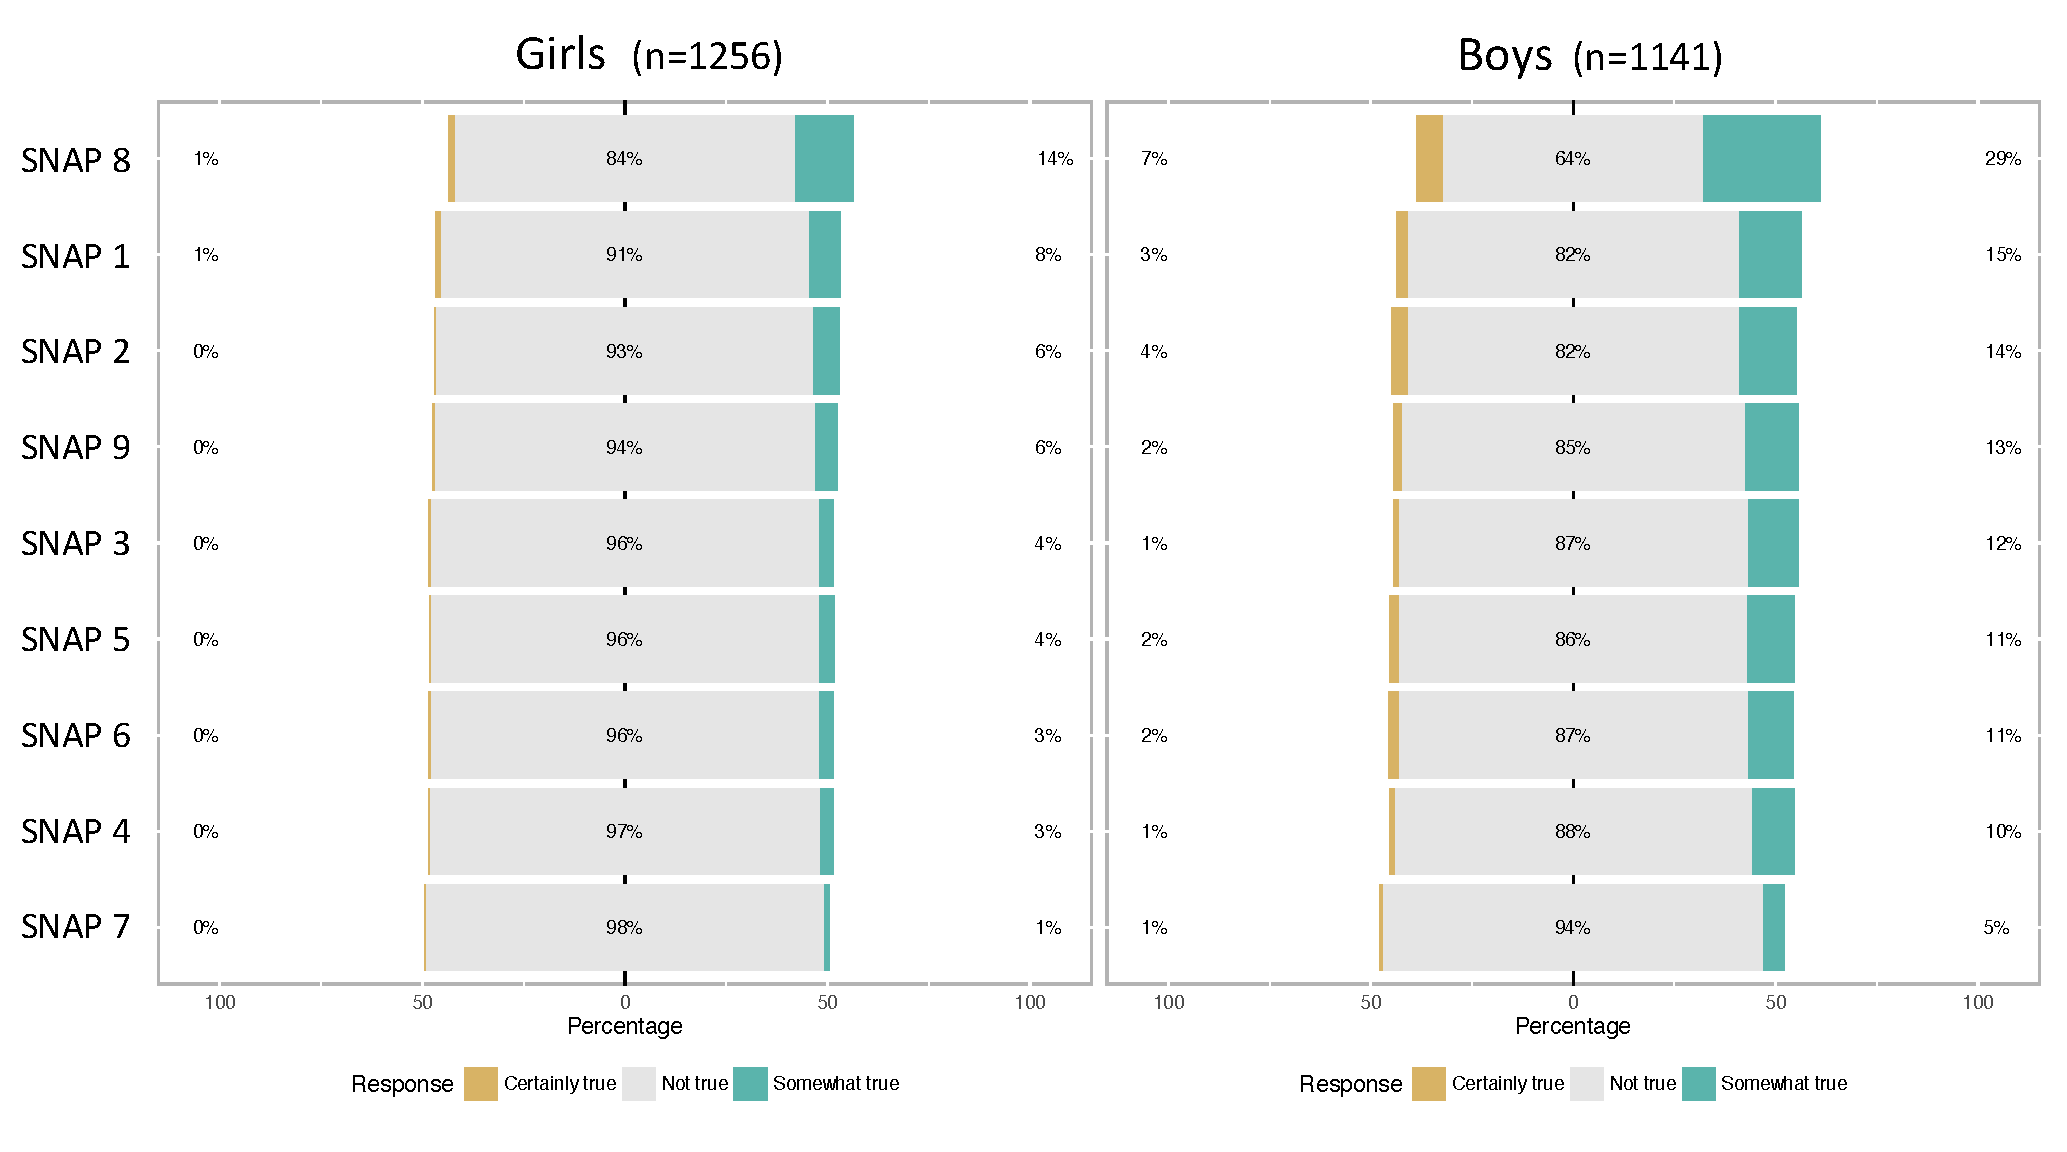
\includegraphics[width=1.05\textwidth]{./Figs/Likert_SNAP_1_9_20160208_pptx.pdf}
\end{tabular}
\caption{The  gender-wise three-level Likert items SNAP 1$, \ldots, $ SNAP 9 sorted according to response pattern.  See 
Fig.~\ref{Data_structure} for explanation of variables.}
\label{Likert_SNAP}
\end{center}
\end{figure}

%To complement Fig.~\ref{Likert_SNAP}, the numerical description of the inattention features are given in Tab.~\ref{Numerical_SNAP}.
 
\begin{table}[H]
\begin{center}
\begin{tabular}{lrrr|rrr|rrr}

  \hline
                & \multicolumn{3}{c|}{\emph{Not true}}  &  \multicolumn{3}{c}{\emph{Somewhat true}}\ &  \multicolumn{3}{|c}{\emph{Certainly true}}\\
                    & All  (\%) & Girls & Boys  & All (\%)  & Girls & Boys & All  (\%) & Girls & Boys\\ 
 \hline                   
      
    SNAP 1  & 86.7 & 91.0 & 81.9**  & 11.3 & 7.6   & 15.4  & 2.0 & 1.3 & 2.7\\ 
    SNAP 2  &88.3 & 93.9   & 82.1** & 9.6 & 5.6 & 14.0 & 2.1 & .5 & 3.9\\ 
    SNAP 3  & 91.8  &  96.6 &  86.6** & 7.6 & 3.2 & 12.4 & .6 & .2 & 1.0 \\ 
    SNAP 4  & 92.5  & 84.4   & 87.4**  & 6.8 & 3.6 & 10.4 & .7& .2 & 1.2 \\ 
    SNAP 5  &  91.4 & 95.9 & 86.3**  & 7.3 & 3.6  & 11.5  &1.3 & .5 & 2.2  \\ 
    SNAP 6  & 91.6 & 96.2 & 86.5**  & 7.1 & 3.4 & 11.5 & 1.3 & .4 & 2.4 \\ 
    SNAP 7  & 96.5 & 98.5   & 94.2**   & 3.0  & 1.2 & 5.1& .5 & .3 & .7 \\ 
    SNAP 8  & 74.8 & 84.3   & 64.4**  & 21.3  & 14.3  & 29.0 &  3.9 & 1.4 & 6.6\\ 
    SNAP 9  & 89.4 & 93.3 & 85.0** & 9.5 & 6.3 & 13.1 & 1.1 & .4  & 1.9 \\ 
        
   \hline
\end{tabular}
\label{Numerical_SNAP}
\end{center}
\caption{Percentage of children obtaining a given response from their teachers on each inattention item (SNAP-IV).
Total number of children = 2397, girls = 1256, boys = 1141.  **: $p$ value $<$.001 according to a chi-square test comparing a ``not true'' report in boys and girls.} 
\end{table}



\subsubsection*{Academic achievement}
Academic achievement scores were provided by the official registers from the Hordaland County. In Norway, secondary schools use a scale spanning from 1 to 6, with `6' being the highest grade (outstanding competence),  `2'  the lowest passing grade (low level of competence), and `1' being a {\it fail}. 
The outcome scores that were available to our study was $average\_grade \in [0, 6]$, the mean value of the grades during the previous semester in high-school (?), comprising all subjects except for physical education (gym). %Figure 1 illustrates results on all variables for all participants included in the present study.  

The distribution of average academic achievement scores are shown in Fig.~\ref{academic_achievement_densities}, separately for girls and boys. 

 \begin{figure}[H]
\begin{center}
\begin{tabular}{ll}
\hspace{-10mm} &
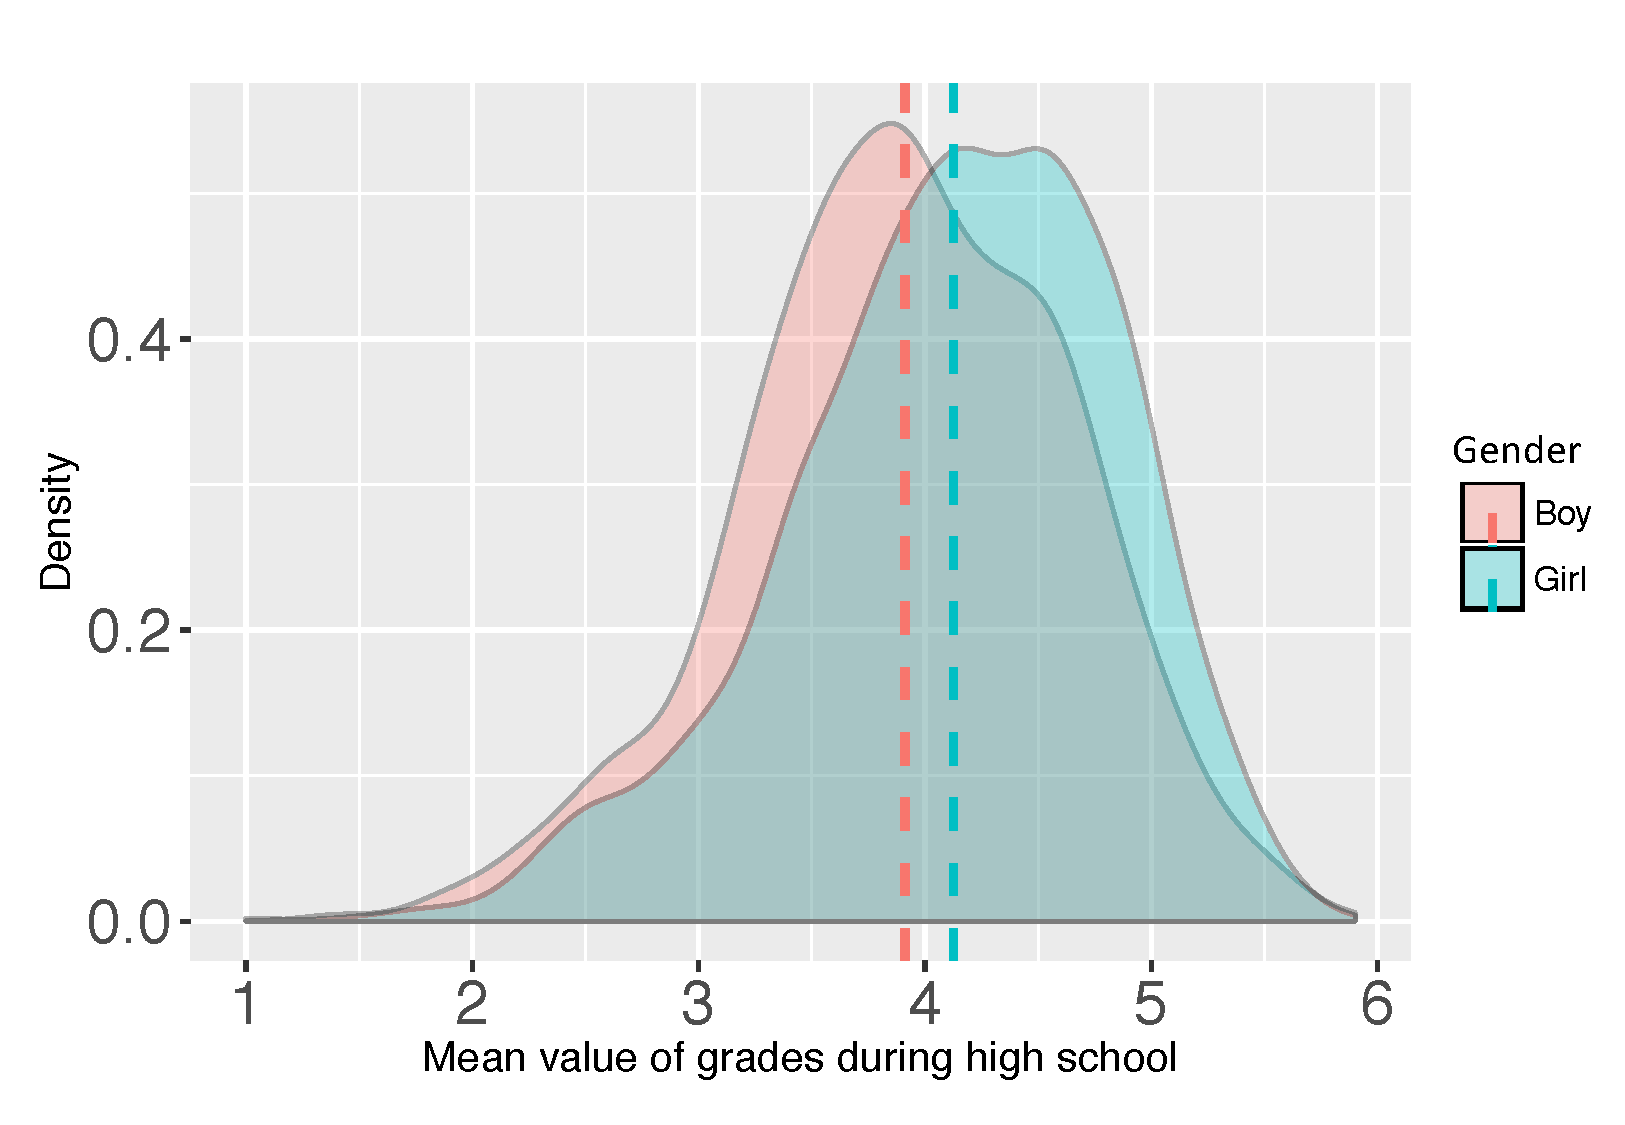
\includegraphics[width=1.05\textwidth]{./Figs/academic_achievement_density_vs_gender_20160208_pptx.pdf}
\end{tabular}
\caption{The  gender-wise distribution of mean academic achievement scores. Vertical dashed lines represent the mean scores for boys ($= 3.91$)
and girls ($= 4.12$), respectively.}
\label{academic_achievement_densities}
\end{center}
\end{figure}


For the present study, the academic achievement scores were categorised into three levels, calculated to generate groups with similar number of participants (see details below). 


\subsection{Pattern analysis and machine learning methods}
The data analysis can be divided into three parts: ({\bf  a}) data preparation, ({\bf b}) explorative data analysis, and ({\bf c}) pattern classification using multivariate statistical methods and machine learning techniques. 

To perform these steps, explained in detail below, we used  {\tt R} (ver. 3.2.3) with selected packages in the 
{\tt RStudio} (ver. 0.99.878) environment, except for Fig.~2
%Figure~\ref{Data_to_classes} 
where {\tt MATLAB} (R2015b) was used. 
Some of the methods were also scripted in {\tt Julia} (version 0.4.2), as a {\tt Jupyter} notebook.
Most of these scripts are available upon request from the last author.
%The data were analysed using R version 3.2.2
% and MATLAB R2016a Prerelease. 
% We applied two categories of statistical methods: (i) descriptive statistics and explorative data analysis, and 
% (ii) classification models with the three intervals of academic achievements as outcome variable, with the nine inattention items, gender and age as predictors. 

%Depiction of the data and the classification methods being used are given in 
%Figure~\ref{Data_to_classes}\footnote{Based on {\tt /Users/arvid/Dropbox/Arvid\_Inattention/code/D\_20151110\_analysis\_20160203.m}  using
%{\tt /Users/arvid/Dropbox/Arvid\_Inattention/data/Dnomiss\_20151110.csv},  and 
%{\tt /Users/arvid/Dropbox/Arvid\_Inattention/manuscript/Figs/Data\_to\_classes\_20151209.pptx}}.\\

\subsubsection*{Data preparation \,  {\footnotesize [{\tt code2/data\_prep\_20160205.R} ; {\tt data\_prep\_and\_visualization\_20160203.m}]}}


The original data was provided as an SPSS file and imported into the R environment. For the analysis we used the sample of $n=2397$ children with complete data 
on $11$ predictor variables and academic achievement as outcome according the data description shown in Fig.~\ref{Data_structure}.

\begin{figure}[H]
\begin{center}
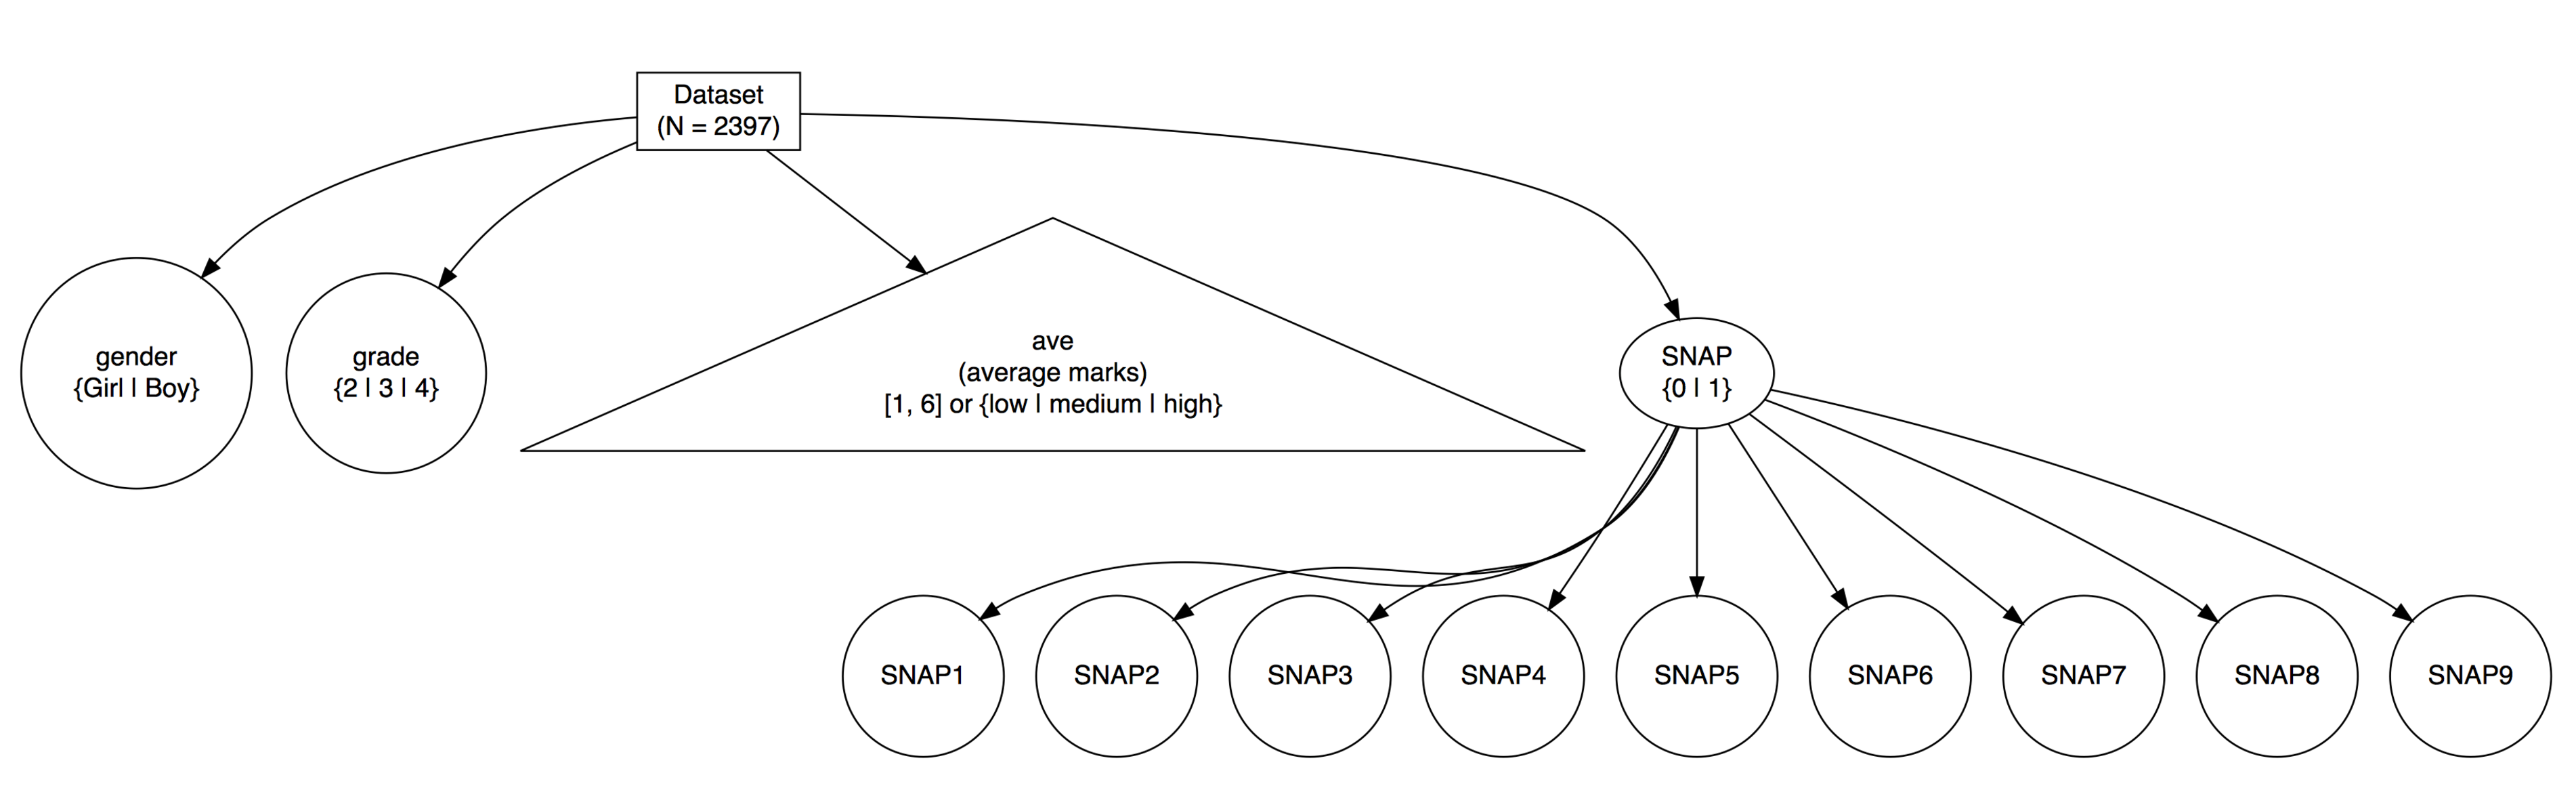
\includegraphics[width=1.00\textwidth]{./Figs/data_prep_structure_grviz_20160203.pdf}
\caption{The data organization for the sample. 
{\it gender} is $0$ (girls) or $1$ (boys), {\it grade} is $2$, $3$, or $4$. The  three-level Likert items from Snap-IV: SNAP1$, \ldots, $ SNAP9 have each three possible values: $0$ (``certainly true''), $1$ (``not true''), and $2$ (``somewhat true''). }
\label{Data_structure}
\end{center}
\end{figure}

% The outcome variables are discretized into $[0.00, 3.75) \mapsto \mbox{\it low}$ ($n_1=779$),  $[3.75,4.43) \mapsto \mbox{\it medium}$ ($n_2=818$),  
% $[4.43, 6.00] \mapsto \mbox{\it high}$ ($n_3=800$). 

For classification purposes, the mean average academic achievement scores were discretised into three intervals (level of academic achievement) constructed such that prior probability was non-informative, i.e. about same number of participants in each outcome category, ignoring gender. These three level ({\small \tt bins} = 3) {\small \tt cutpoints} for the mean average academic achievement score {\small \tt aver}  was obtained as:  {\small \tt cutpoints<-quantile(aver,(0:bins)/bins)}.

By this we obtained the following levels and intervals:
{\it low}: $[1.000, 3.750)$  ($n_{\mbox{\tiny low}} = 779$); 
{\it medium}: $[3.750, 4.429)$  ($n_{\mbox{\tiny medium}} = 818$); 
{\it high}: $[4.429, 5.900)$  ($n_{\mbox{\tiny high}} = 800$); 


Depiction of the data values and the classification methods being used are given in Fig.~\ref{Data_to_classes}.


 
 \begin{figure}[H]
\begin{center}
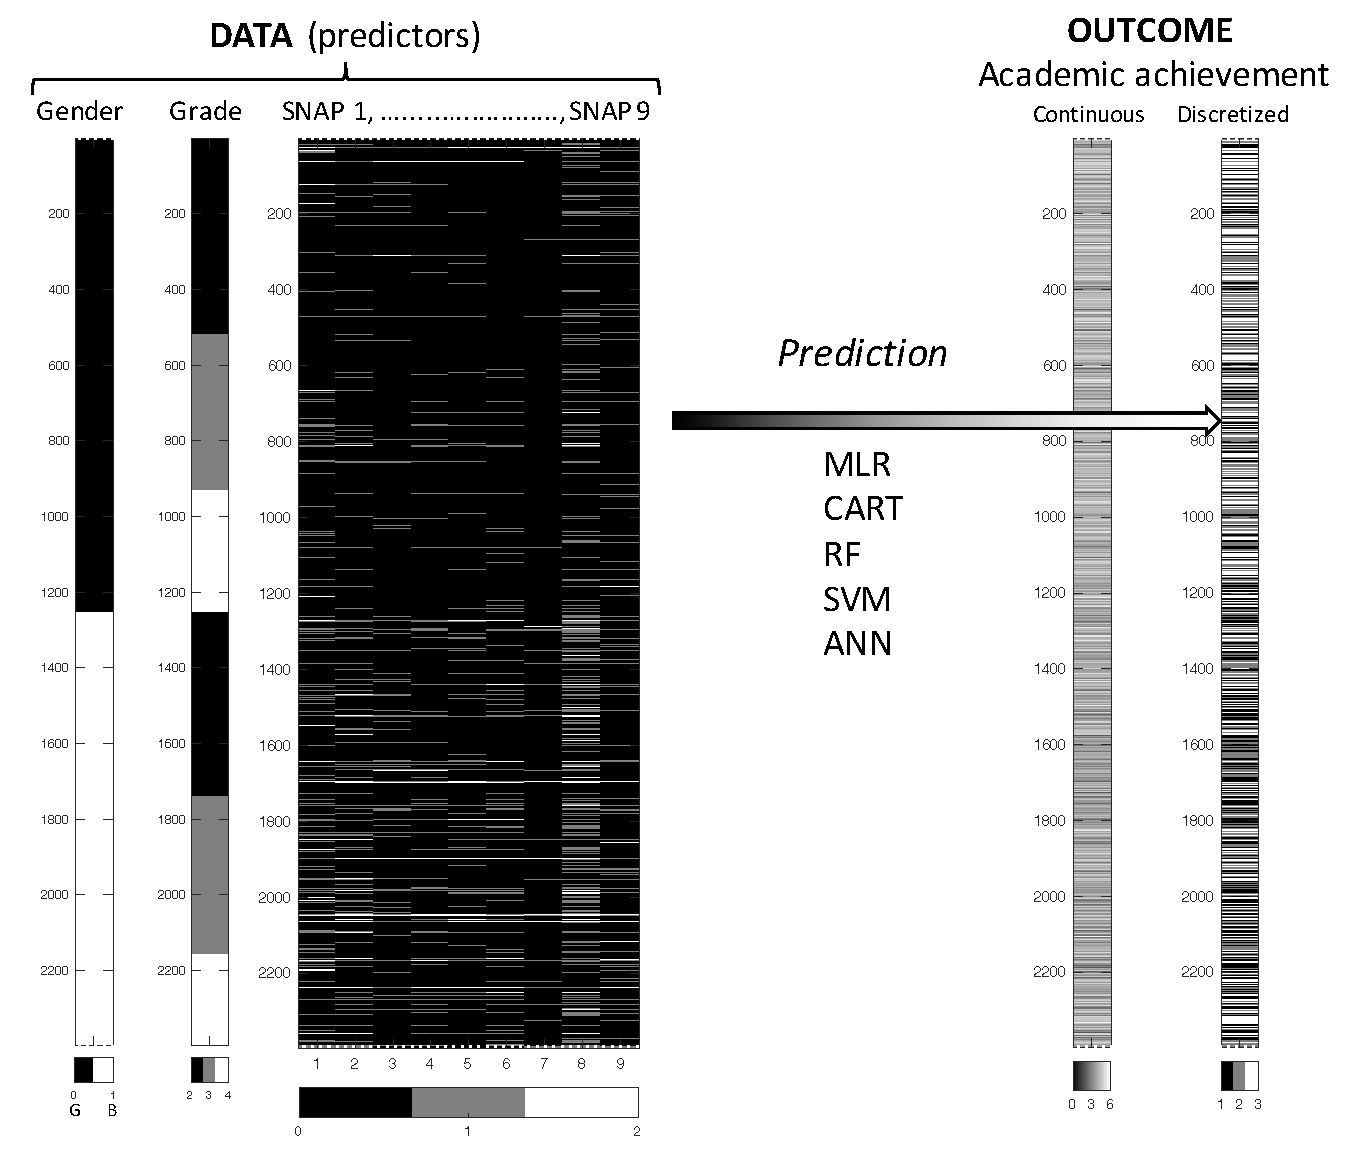
\includegraphics[width=0.85\textwidth]{./Figs/Data_to_classes_20160205_pptx.pdf}
\caption{The predictor data (explanatory variables), the academic achievement outcome, and the types of classification analyses being performed. See 
Fig.~\ref{Data_structure} for explanation of variables.\,
MLR = Multinomial logistic regression, CART = Classification and regression trees, 
RF = Random forest ensemble learning, SVM = Support vector machines, ANN = Artificial neural networks. }
\label{Data_to_classes}
\end{center}
\end{figure}




% OVERALS, categorical CCA with optimal scaling approach
% http://stats.stackexchange.com/questions/131375/explanatory-variables-with-linear-discriminant-analysis

%\subsubsection*{Explorative data analysis  \,  {\footnotesize [{\tt code2/explorative\_data\_analysis\_20160208.R]}}}
%Sex differences in age, the total inattention score, and the total academic achievement score were compared using parametric tests and sex differences on the single inattention items by non-parametric tests.
% 
%
% \begin{figure}[H]
%\begin{center}
%\begin{tabular}{ll}
%\hspace{-10mm} &
%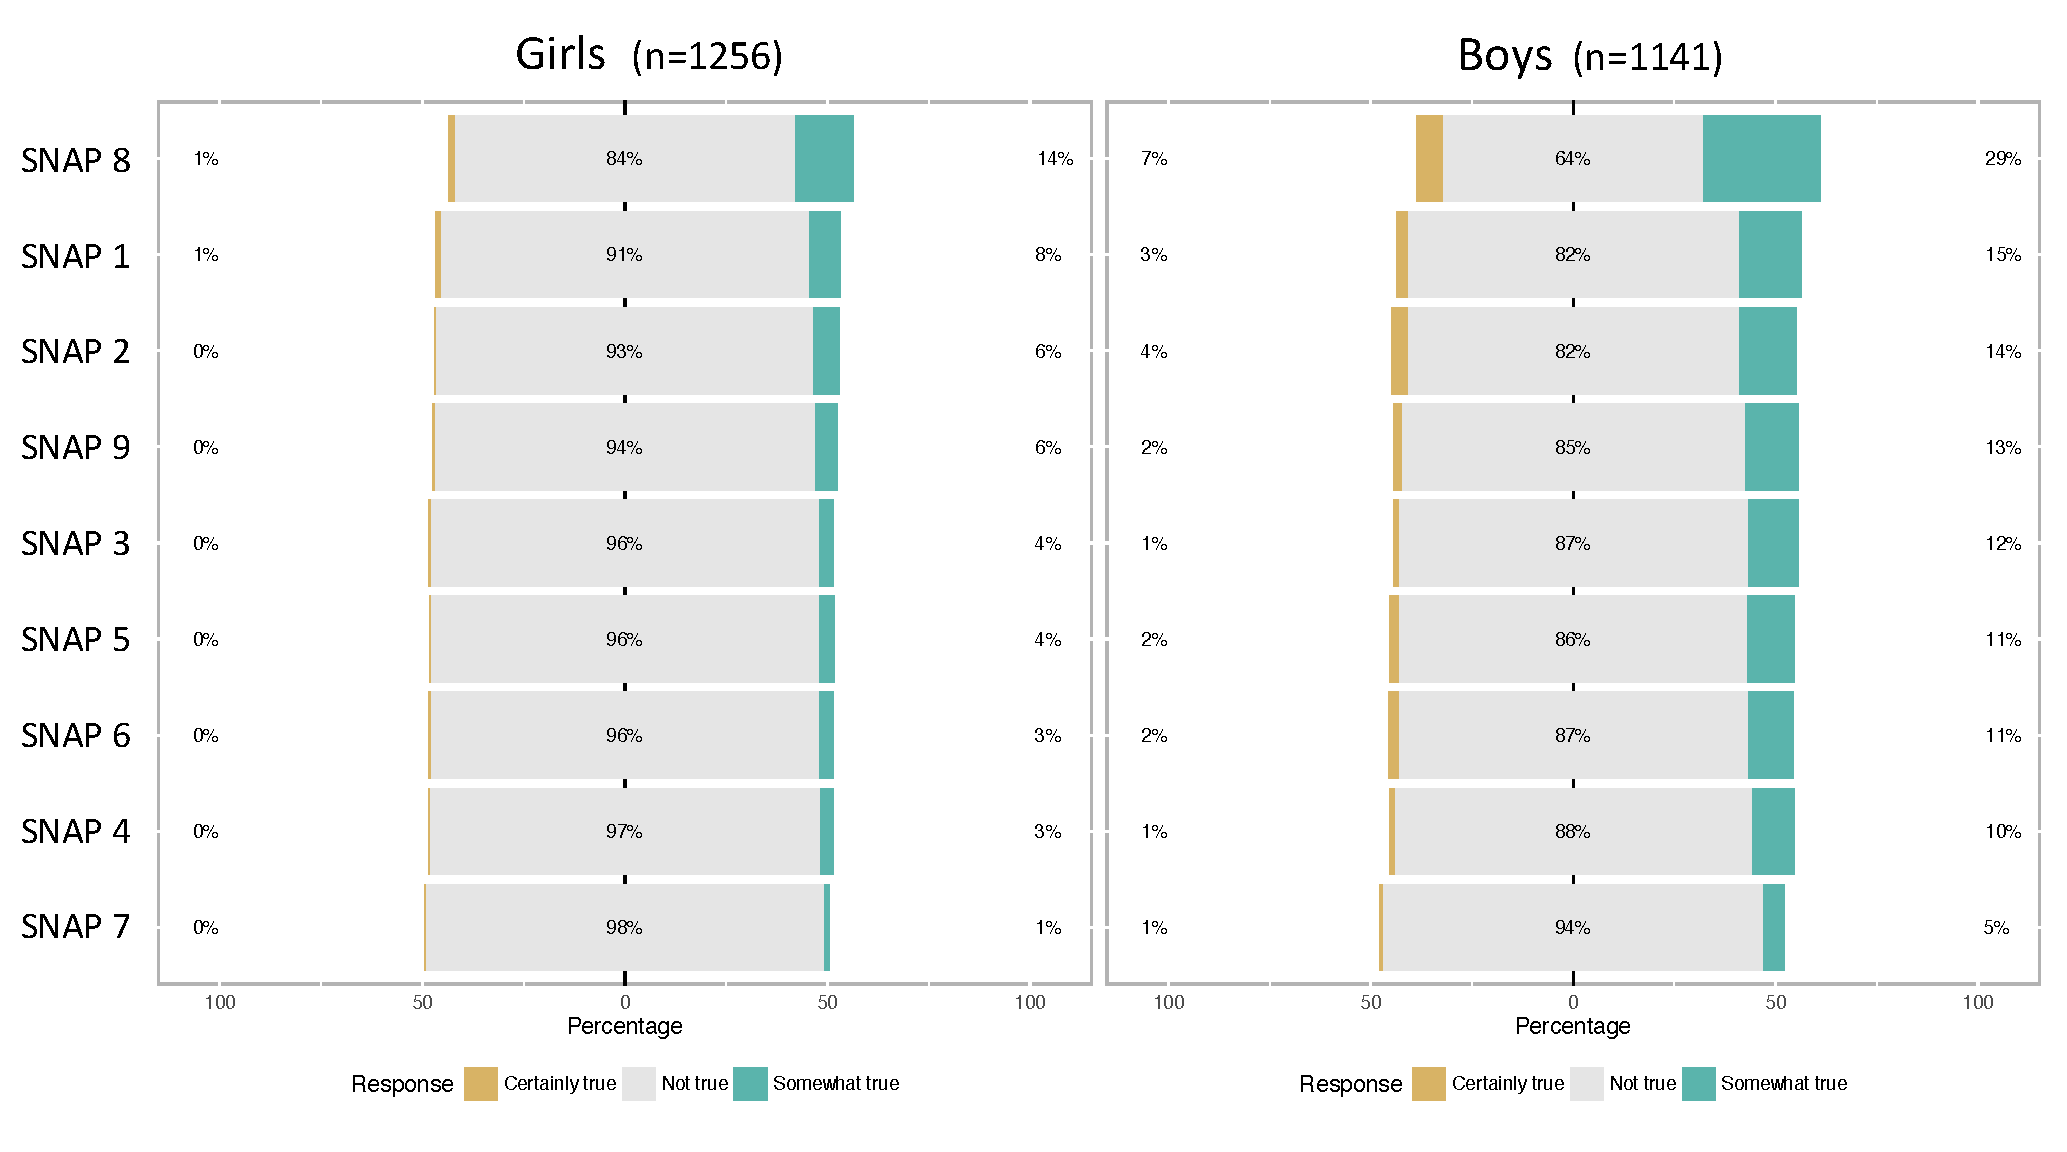
\includegraphics[width=1.05\textwidth]{./Figs/Likert_SNAP_1_9_20160208_pptx.pdf}
%\end{tabular}
%\caption{The  gender-wise three-level Likert items SNAP 1$, \ldots, $ SNAP 9 sorted according to response pattern.  See 
%Fig.~\ref{Data_structure} for explanation of variables.}
%\label{Likert_SNAP}
%\end{center}
%\end{figure}
%
%To complement Fig.~\ref{Likert_SNAP}, the numerical description of the inattention features are given in Tab.~\ref{Numerical_SNAP}.
% 
%\begin{table}[H]
%\begin{center}
%\begin{tabular}{lrrr|rrr|rrr}
%
%  \hline
%                & \multicolumn{3}{c|}{\emph{Not true}}  &  \multicolumn{3}{c}{\emph{Somewhat true}}\ &  \multicolumn{3}{|c}{\emph{Certainly true}}\\
%                    & All  (\%) & Girls & Boys  & All (\%)  & Girls & Boys & All  (\%) & Girls & Boys\\ 
% \hline                   
%      
%    SNAP 1  & 86.7 & 91.0 & 81.9**  & 11.3 & 7.6   & 15.4  & 2.0 & 1.3 & 2.7\\ 
%    SNAP 2  &88.3 & 93.9   & 82.1** & 9.6 & 5.6 & 14.0 & 2.1 & .5 & 3.9\\ 
%    SNAP 3  & 91.8  &  96.6 &  86.6** & 7.6 & 3.2 & 12.4 & .6 & .2 & 1.0 \\ 
%    SNAP 4  & 92.5  & 84.4   & 87.4**  & 6.8 & 3.6 & 10.4 & .7& .2 & 1.2 \\ 
%    SNAP 5  &  91.4 & 95.9 & 86.3**  & 7.3 & 3.6  & 11.5  &1.3 & .5 & 2.2  \\ 
%    SNAP 6  & 91.6 & 96.2 & 86.5**  & 7.1 & 3.4 & 11.5 & 1.3 & .4 & 2.4 \\ 
%    SNAP 7  & 96.5 & 98.5   & 94.2**   & 3.0  & 1.2 & 5.1& .5 & .3 & .7 \\ 
%    SNAP 8  & 74.8 & 84.3   & 64.4**  & 21.3  & 14.3  & 29.0 &  3.9 & 1.4 & 6.6\\ 
%    SNAP 9  & 89.4 & 93.3 & 85.0** & 9.5 & 6.3 & 13.1 & 1.1 & .4  & 1.9 \\ 
%        
%   \hline
%\end{tabular}
%\label{Numerical_SNAP}
%\end{center}
%\caption{Percentage of children obtaining a given response from their teachers on each inattention item (SNAP-IV).
%Total number of children = 2397, girls = 1256, boys = 1141.  **: $p$ value $<$.001 according to a chi-square test comparing a ``not true'' report in boys and girls. [\color{blue}{Astri check this - in R?} ]}
%\end{table}
%
%
%The distribution of average academic achievement scores are shown in Fig.~\ref{academic_achievement_densities}, separately for girls and boys. 
%
% \begin{figure}[H]
%\begin{center}
%\begin{tabular}{ll}
%\hspace{-10mm} &
%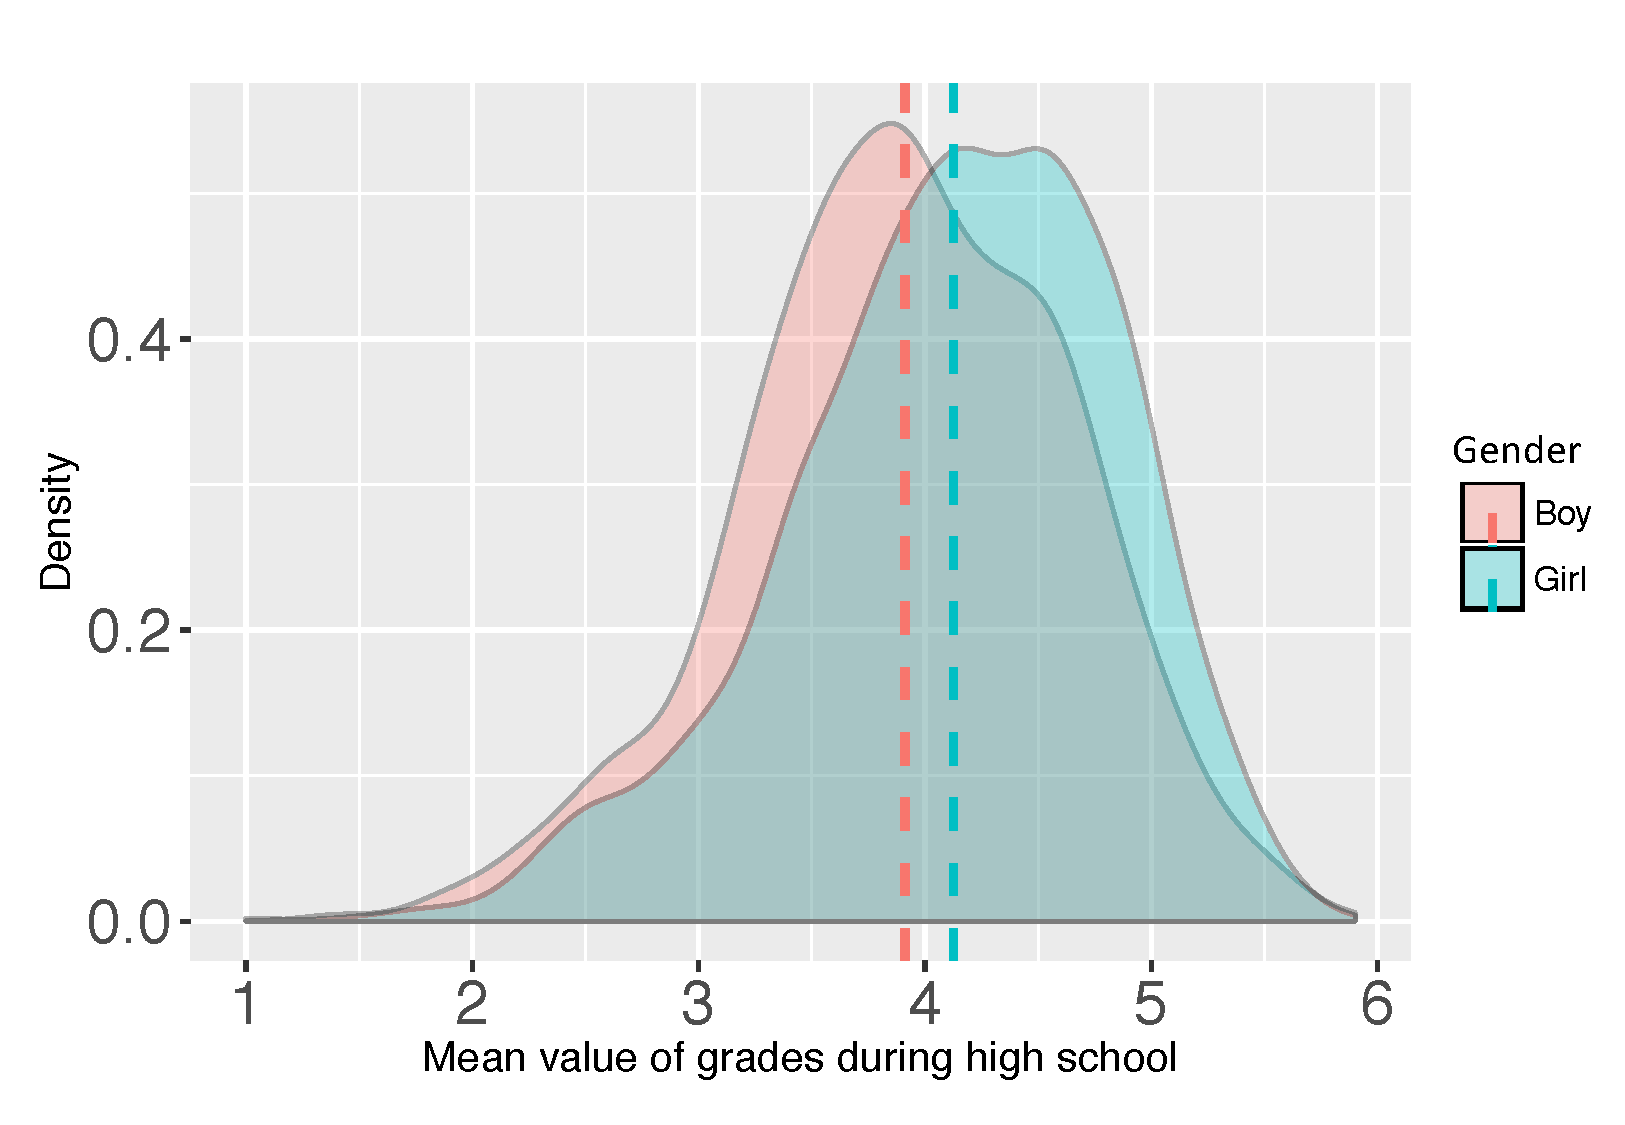
\includegraphics[width=1.05\textwidth]{./Figs/academic_achievement_density_vs_gender_20160208_pptx.pdf}
%\end{tabular}
%\caption{The  gender-wise distribution of mean academic achievement scores. Vertical dashed lines represent the mean scores for boys ($= 3.91$)
%and girls ($= 4.12$), respectively.}
%\label{academic_achievement_densities}
%\end{center}
%\end{figure}
%



% Check out:
% Working with categorical data with R and the vcd and vcdExtra packages
% Michael Friendly York University, Toronto
% Using vcdExtra version 0.5-8 and vcd version 1.2-13; Date: 2013-06-26

% and the survey  surveydata packages


%\subsubsection{General linear model (GLM)}
%
%The general linear model, in our case  ordinary least-squares, model the outcome variable $y$ (mean academic achievment) as a linear 
%combination of a set of explanatory variables $x_1, \ldots, x_p$, i.e.
%\begin{equation}
%\label{eq_GLM}
%y = \beta_{0} + \beta_{1} x_1 + \cdots + \beta_{p} x_p
%\end{equation}
%where $x_1 = \mbox{\it Gender}$,  $x_2 = \mbox{\it Grade}$, and $x_3 = \mbox{\it SNAP1}, \ldots, x_{11} = \mbox{\it SNAP9}$.

\subsubsection*{Multinomial logistic regression model (MLR)}
Multinomial logistic regression is used in the present study where we include a set of explanatory variables on a nominal level - the three levels of academic achievement scores - and the nine inattention items, gender and age as predictors. It is exploratory, in that we have no prior assumption regarding the weights of these items. In other words, the analysis investigates if a prediction can come from one or a limited set of items. 
To obtain this, the multinomial logistic regression model relates a set of explanatory variables $x_1, \ldots, x_p$ to a set of log-odds $\log(\pi_2/\pi_1), \ldots \log(\pi_J/\pi_1)$ according to
\begin{equation}
\label{eq_MLR}
\log(\pi_j/\pi_1) = \beta_{j0} + \beta_{j1} x_1 + \cdots + \beta_{jp} x_p
\end{equation}
for $j=2,\ldots,J$. Here, $j = 1$ represents the base level category, $\pi_j = P(\mbox{academic achievement level} = j)$, $\pi_j/\pi_{j'}$ denotes the odds of category $j$ relative to $j'$, and $\sum_{j=1}^J \pi_j = 1$ (see e.g. \cite{Bilder2015} for details).
In our case, we let the base level category $j=1$ be the {\it high} (=3) mean academic achievement.
For computations we used the {\tt multinom()} function in the R package {\tt nnet}. \\
%For category (ii) the outcome variable academic achievement was defined in the interval $[0, 6]$ as mean average marks.  For category (iii) the mean average marks were discretized into three intervals {\it low} ($1$), {\it medium} ($2$), and {\it high} ($3$) constructed from the data to have uniform sample distributions. 


%\subsubsection{Descriptive and explorative data analysis (EDA)}
%Sex differences in age, the total inattention score, and the total academic achievement score were compared compared using parametric tests and sex differences on the single inattention items by non-parametric tests.
% 
% 
%%\subsubsection{General linear model (GLM)}
%%
%%The general linear model, in our case  ordinary least-squares, model the outcome variable $y$ (mean academic achievment) as a linear 
%%combination of a set of explanatory variables $x_1, \ldots, x_p$, i.e.
%%\begin{equation}
%%\label{eq_GLM}
%%y = \beta_{0} + \beta_{1} x_1 + \cdots + \beta_{p} x_p
%%\end{equation}
%%where $x_1 = \mbox{\it Gender}$,  $x_2 = \mbox{\it Grade}$, and $x_3 = \mbox{\it SNAP1}, \ldots, x_{11} = \mbox{\it SNAP9}$.
%
%\subsubsection{Multinomial logistic regression model (MLR)}
%Multinomial logistic regression is used in the present study where we include a set of explanatory variables on a nominal level - the three levels of academic achievement scores - and the nine inattention items, gender and age as predictors. It is exploratory, in that we have no prior assumption regarding the weights of these items. In other words, the analysis investigates if a prediction can come from one or a limited set of items. 
%To bobtain this, the multinomial logistic regression model relates a set of explanatory variables $x_1, \ldots, x_p$ to a set of log-odds $\log(\pi_2/\pi_1), \ldots \log(\pi_J/\pi_1)$ according to
%\begin{equation}
%\label{eq_MLR}
%\log(\pi_j/\pi_1) = \beta_{j0} + \beta_{j1} x_1 + \cdots + \beta_{jp} x_p
%\end{equation}
%for $j=2,\ldots,J$. Here, $j = 1$ represents the base level category, $\pi_j = P(\mbox{academic achievement level} = j)$, $\pi_j/\pi_{j'}$ denotes the odds of category $j$ relative to $j'$, and $\sum_{j=1}^J \pi_j = 1$ (see e.g. \cite{Bilder2015} for details).
%In our case, we let the base level category $j=1$ be the {\it high} (=3) mean academic achievement.
%For computations we used the {\tt multinom()} function in the R package {\tt nnet}. \\



%\subsubsection{Linear discriminant analysis (DISCR)}

\subsubsection*{Classification trees (CART)}

The Snap-IV items were included together with age and gender as predictor variables in a conditional inference trees analysis (CART; Hothorn et al., 2006)  with academic achievement level as the outcome variable by using  the  the R-package party: A Laboratory for Recursive Partytioning, including conditional inference trees (\textbf{ctree}) and conditional inference forests (\textbf{cforest}). trees (\textbf{mob}) \cite{Strobl2009}. This particular kind of analysis takes into account the distributional properties of the measures. The conditional inference model states, that if the null hypothesis of there being independence between any of the covavariates and the response cannot be rejected, the variable in question is excluded from further exploration. However, when one variable distinguishes itself by having the strongest association with the response, a split is created with two disjoint sets of the variable in question. The Bonferroni adjusted p value of the split value is calculated. For each such node, the abovementioned procedure is repeated until none of the covariates can reject the null hypothesis. From these models we expect to find a cluster of items with a strong weight in predicting academic outcome, and that clusters of some of these variables will be generated from both methods and from the previous factor analysis.

%The nine Snap-IV variables representing externalizing behaviour are included in a second set of analyses to investigate  their influence on the importance of the inattention variables in explaining academic achievement.  \\

%The Gini importance is included in the present study. This is a weighted measure of the mean improvement in the splitting criterion for all its positions in the forest. This is thus a more elaborate variable than counting the number of times a variable is selected cross the ensemble of trees \cite{Stroble2009}. 
%"Gini importance
%Every time a split of a node is made on variable m the gini impurity criterion for the two descendent nodes is less than the parent node. Adding up the gini decreases for each individual variable over all trees in the forest gives a fast variable importance that is often very consistent with the permutation importance measure.". http://stats.stackexchange.com/questions/92419/relative-importance-of-a-set-of-predictors-in-a-random-forests-classification-in
%
%For the impurity measure: "at each split, you can calculate how much this split reduces node impurity (for regression trees, indeed, the difference between RSS before and after the split). This is summed over all splits for that variable, over all trees."
%


\subsubsection*{Random forest ensemble learning (RF)}

Random forest (RF) is an ensemble machine learning algorithm, which is 
best defined as a "combination of tree predictors such that each tree depends 
on the values of a random vector sampled 
independently and with the same distribution for all trees in the forest" \cite{Breiman2001}.
For classification problems, the forest prediction
is the unweighted plurality of class votes, where the algorithm converges with a large 
enough number of trees.
\begin{comment}
 ($k \rightarrow \infty$).
\begin{equation}
      f(x,T,\theta_k),  \, \, k=1,2,...,K,
\end{equation}     
where $\theta_k$  are random vectors that meet i.i.d (independent and identically 
distributed) assumption (6).  For classification problems, the forest prediction
is the unweighted plurality of class votes. The algorithm converges with a large 
enough number of trees ( $k \rightarrow \infty$ ) (5).\\
\end{comment}

For the classification of demographic ({\it Gender} and {\it Grade}) and the nine Snap-IV items, giving the feature vectors $x_1, x_2, \ldots, x_{11}$ defined above, 
into our set of academic achievement labels
 ${\cal C} = \{\text{\it low}, \text{\it medium}, \text{\it high}\}$, 
we used the Breiman RF ensemble learning algorithm \cite{Breiman2001} as implemented in the R package {\tt randomForest}. 
In this setting we are given a set of training data ${\cal D} = \left\{(\mathbf{v}^i, c^i)\right\}_{i=1,\ldots,n}$ 
(to be defined below).
The classification task is then to learn a general mapping from
previously unseen test data to their corresponding class labels, i.e. $c: \mathbf{R}^d \rightarrow {\cal C}$, where $d=11$ in our case.
More specifically, adopting the notation in \cite{Criminisi2013},
let  $\mathbf{v} = (x_1,\ldots,x_d) \in \mathbf{R}^d$ denote the input data feature vector (predictor), and let $c \in {\cal C}$ denote the output academic achievement 
label (response). 
The RF algorithm incorporate a collection of binary classification trees indexed by $t=1,\ldots,n_{\text{tree}}$. Each classification tree is characterised by its input root node, 
internal split nodes,  and its leaf terminal nodes containing class labels. 

In this setting, the RF algorithm can be briefly described as follows: (i) Draw $n_{\text{tree}}$ samples from the original data ${\cal D}$, using
random sampling with replacement; (ii) For each bootstrap sample, grow a classification tree such that for each node: randomly sample $m_{\text{try}}$ of the predictor variables
and chose the "best split" (Gini criterion to be defined below) from among those feature variables ($1 \leq m_{\text{try}} \ll d$). The  largest tree possible is grown and is not pruned. Using only
$m_{\text{try}}$ of the predictor variables selected at random is
in contrast to standard tree classification (CART), where each node is split using the best split among all $d$ variables.
(iii) The forest consists of $n_{\text{tree}}$ trees. Each tree gives a classification for a given data point. Predict new data point $\mathbf{x}$  by putting $\mathbf{x}$  down each of the 
$n_{\text{tree}}$ trees and make a majority vote for classification across the forest.

For a given tree, we let ${\cal S}_0$  denote the set of input predictor data 
vectors that is fed into the root node, ${\cal S}_j$ the subset of data points reaching node $j$ in the binary splitted tree, and $\{{\cal S}_j^L, {\cal S}_j^R\}$ denote the subsets of data points
that reaches the left and right child, respectively, of node $j$,  where ${\cal S}_j^L \cup {\cal S}_j^R = {\cal S}_j$ and ${\cal S}_j^L \cap {\cal S}_j^R = \emptyset$.
 In the "off-line" tree training, each split node $j$ is associated with a parameter vector $\boldsymbol{\theta}_j$ that is trained by optimizing an
objective function $I$ (defined below), i.e. $\boldsymbol{\theta}_j = \arg \max_{\boldsymbol{\theta} \in {\cal T}_j}  I({\cal S}_j, \boldsymbol{\theta})$. 

In this notation,
a binary-valued test function $h(\mathbf{v},\boldsymbol{\theta}_j): \boldmath{R}^d \times {\cal T} \rightarrow  \{0 , 1\}$ is applied at each split node $j$.
Here, $0$ and $1$ denote "true" and "false", respectively, and the data point $\mathbf{v}$ arriving at split node $j$ is sent to its left ($0$) or right ($1$) child node, accordingly. 
${\cal T}$ is the set of all possible split function parameters, and ${\cal T}_j \subseteq {\cal T}$ is the subset of parameters available at node $j$. We thus have
${\cal S}_j^L({\cal S}_j, \boldsymbol{\theta}) = \left\{(\mathbf{v}, c) \in {\cal S}_j \mid h(\mathbf{v},\boldsymbol{\theta}) = 0\right\}$ and 
${\cal S}_j^R({\cal S}_j, \boldsymbol{\theta}) = \left\{(\mathbf{v}, c) \in {\cal S}_j \mid h(\mathbf{v},\boldsymbol{\theta}) = 1\right\}$.

The objective function being used was the Gini index, i.e. $I = i(\tau) = 1 - \sum_{c \in {\cal C}} p_c^2$, measuring the likelihood that a data  point would be incorrectly labeled
if it was randomly classified according to the distribution of class labels within the node. The optimal binary split is then the one that maximises the 
improvement in the Gini index.

Proximity, $P(i,j)$  in the RF model is the proportion how often two data points (rows), $i$ and $j$ end in the same leaf node for 
different trees. 
{\it Outliers} are defined as cases having small proximities to all other cases. Since the data in some classes is more spread out than
others, outlyingness is defined only with respect to other data in the same class as the given case. More specifically,
for a given case $i$  let $out(i) = 1/A_i$, where 
\begin{displaymath}
A_i = \sum_{\mbox{\scriptsize $k$ in same class as $i$}} P(i, k)^2
\end{displaymath}
For all $i$ in the same class, let the mean absolute deviation $MAD =  \frac{1}{n} \sum_{i=1}^{n} |out(i) - med|$ , where $med$ is the median of $out(i)$
for all $i$ in the same class. The outlyingness of a case $i$ is then the $MAD$-normalized measure, $outlyingness(i) = \max \left\{(out(i) - med) / MAD, 0 \right\}$. 


\subsubsection*{Support vector machine (SVM)}

Support vector machines (SVMs) are supervised models with an aim to learn structures in the data, here by including the tree categories of academic achievement level as outcome variable, and learning algorithms to learn how these categories can be explained from information about teacher reports on the nine inattention items, age and sex. A training set is selected where the participants are marked for belonging to one of the three categories, a model is built by the SVM training algorithm to assign new participants into one of the categories. The SVM model is mapped as points in space, where the three categories are divided as clearly as possible. New examples are then predictied to belong to one of these categories depending on the side if the gap they fall on. In the present study we use a non-linear classification using the kernel trick, where the input is mapped into high-dimensional feature spaces. 



\subsubsection*{Artificial neural networks  (ANN)}
Artificial neural networks (ANN) method is another machine learning technique inspired by biological neural networks. Like in biology, the method present the results as interconnected "neurons" that may exchange information between each other. They may both have different weighs and are adaptive and therefore capable of learning. In the present study, the method is appropriate, because a category belonging can be dependent on several variables. In this model, these variables are processing elements or "neurons" that are connected together to form a network. In the present study the neural network model is thus used to classify patterns of inattention and the sequence of their weights, and by this probably detect novel associations. 

\section{RESULTS}


\begin{comment}
 % ----------------------------------------------------------------------------------------------------------------------------
 
\subsection{Descriptive and explorative data analysis (EDA)}

\subsubsection*{Demographics, SNAP scores and academic achievements}
Restricting the participants to the ones with information on all nine teacher reported inattention items from SNAP-IV and information about academic achievement included 2603 individuals, 52.2\% girls. Mean age when included in wave 4 was 17.5 (sd = .84), with a non-significant difference between girls ( ) and boys ( ). \\
%There is a high correspondence between class grade when attending primary school and  when attending high school, with 98.3\% attending lowest levels at both time points, 95.3\% at the second and 90.8\% at the third levels (Table 1). 
%Among the 48 adolescents attending lower level than expected in the latter group, 34 are boys. 
%The academic achievement scores in the whole sample are not significantly different between the adolescents attending the second, third or fourth grade as reported by their primary school teachers, but girls obtain significantly higher scores when evaluated in the second than fourth grade (F(1,691.7) = 2.32, $p$ = .021. No statistically significant differences between the three high school classes are found when analysing the full sample, but within the gender groups, the academic scores are statistically significant  higher in the first than third year for girls, $t$ (1, 633.9) = 2.6, $p$ = .009, and significantly higher in the third than in the second year for boys, $t$(1, 381.6) = -2.04, $p$ = .47.  (see Table 1).  

Overall, girls (mean = 4.13, SD = .72) showed significantly higher academic scores than the boys (mean = 3.91, sd = .72, $t$(1,2395)=7.2, $p$ $<$ .001),. The distribution was close to normal withnin both gender groups, with a small shift towards the highest leve in the girls (Figure 3). The age range was ............, with a non-significant difference between girls and boys.\\

Most children were rated without inattention problems according to the SNAP-IV items, with statistically significant lower percentages in boys than girls on most items (Table 1). The strongest gender difference was found on the item reflecting distractibility (\emph{Often is distracted by extraneous stimuli}, item 8), where teachers reported that this was somewhat true for 29\% and true for 6.6\% of the boys. Although lower percentages were reported within these categories for girls, distractibility was the problem most frequently reported by teachers for both genders. 

 % ----------------------------------------------------------------------------------------------------------------------------
\end{comment}

%\newpage




%\begin{figure}[htbp]
%\centering
%\includegraphics{astri_wave1_inattention_cond_infer_trees_20150502_files/figure-latex/unnamed-chunk-9-1.pdf}
%\caption{}
%\end{figure}




%\subsubsection*{Primary school teacher's reports on the SNAP-IV items}
% \subsection{Regression models}
% 
% 
% \subsubsection{General linear model (GLM)}
% 
% %\subsubsection*\bf{GLM}
%The first fitted model is a general linear regression model, including a continuous score of academic achievement as outcome variable, with gender, grade and the nine SNAP inattention variables as predictors, i.e. ({\small \tt General\_Linear\_Models\_20151211.R})
% \begin{footnotesize}
%\begin{shaded}
%\begin{verbatim}
%X <- read.csv("../data/X.csv", header = TRUE, sep = ",")
%Yc <- read.csv("../data/Yc.csv", header = TRUE, sep = ",")
%D <- cbind(X, Yc)
%D.lm.1 <- lm(AverageMarks ~ Gender+Grade +
%                 SNAP1+SNAP2+SNAP3+SNAP4+SNAP5+SNAP6+SNAP7+SNAP8+SNAP9,
%                 data = D)
%library(xtable)
%xtable(D.lm.1)
%xtable(anova(D.lm.1))
%library(stargazer)
%stargazer(D.lm.1)
%stargazer(anova(D.lm.1))
%\end{verbatim}
%\end{shaded}
%\end{footnotesize}
%Table~\ref{LM_results_test} shows that the full model was statistically significant, explaining about 10\% of the variance in the outcome variable. Gender and SNAP 2 and 8, reflecting problems related to sustained attention and distractibility, were highly statistically significant (\emph{Often is distracted by extraneous stimuli}  and \emph{often has difficulty sustaining attention in tasks or play activities} ($p$ $=$ .001)).  Although at a lower level, both SNAP 1 (\emph{Often fails to give close attention to details or makes careless mistakes in schoolwork, work, or other activities}) and grade turned out to be statistically significant.\\
% 
% \begin{comment}
%\emph{Coefficients}:\\
%             Estimate Std. Error t value Pr($>$$|t|$) \\  
%(Intercept)  4.294153   0.055312  77.635  < 2e-16 ***\\
%gender      -0.115459   0.029316  -3.938 8.44e-05 ***\\
%grade       -0.037753   0.018087  -2.087  0.03696 *  \\
%snap1       -0.112791   0.041374  -2.726  0.00645 ** \\
%snap2       -0.284644   0.057071  -4.988 6.56e-07 ***\\
%snap3       -0.006396   0.057531  -0.111  0.91149    \\
%snap4        0.063324   0.071450   0.886  0.37557    \\
%snap5        0.106937   0.064354   1.662  0.09670 . \\ 
%snap6       -0.104551   0.061290  -1.706  0.08817 .  \\
%snap7        0.026197   0.079237   0.331  0.74096    \\
%snap8       -0.191189   0.037535  -5.094 3.79e-07 ***\\
%snap9       -0.031721   0.048218  -0.658  0.51069    \\
%---
%Signif. codes:  0 �***� 0.001 �**� 0.01 �*� 0.05 �.� 0.1 � � 1\\
%
%Residual standard error: 0.6923 on 2385 degrees of freedom\\
%Multiple R-squared:  0.1044,	Adjusted R-squared:  0.1003 \\
%F-statistic: 25.28 on 11 and 2385 DF,  p-value: $<$ 2.2e-16\\
%\end{comment}
%
%
%
%% > xtable(D.lm.1)
%% latex table generated in R 3.2.2 by xtable 1.8-0 package
%% Sat Dec 12 06:38:44 2015
%\begin{table}[H]
%  \caption{Results from  the general linear model, {\tt lm()}.} 
%  \label{LM_results_test}
%\centering
%\begin{tabular}{rrrrr}
%  \hline
% & Estimate & Std. Error & t value & Pr($>$$|$t$|$) \\ 
%  \hline
%(Intercept) & 4.2942 & 0.0553 & 77.63 & 0.0000 \\ 
%  Gender & -0.1155 & 0.0293 & -3.94 & 0.0001 \\ 
%  Grade & -0.0378 & 0.0181 & -2.09 & 0.0370 \\ 
%  SNAP1 & -0.1128 & 0.0414 & -2.73 & 0.0065 \\ 
%  SNAP2 & -0.2846 & 0.0571 & -4.99 & 0.0000 \\ 
%  SNAP3 & -0.0064 & 0.0575 & -0.11 & 0.9115 \\ 
%  SNAP4 & 0.0633 & 0.0715 & 0.89 & 0.3756 \\ 
%  SNAP5 & 0.1069 & 0.0644 & 1.66 & 0.0967 \\ 
%  SNAP6 & -0.1046 & 0.0613 & -1.71 & 0.0882 \\ 
%  SNAP7 & 0.0262 & 0.0792 & 0.33 & 0.7410 \\ 
%  SNAP8 & -0.1912 & 0.0375 & -5.09 & 0.0000 \\ 
%  SNAP9 & -0.0317 & 0.0482 & -0.66 & 0.5107 \\ 
%   \hline
%\end{tabular}
%% From stargazer(D.lm.1)
%\begin{tabular}{@{\extracolsep{5pt}}lc} 
%\hline \\[-1.8ex] 
%Observations & 2,397 \\ 
%R$^{2}$ & 0.104 \\ 
%Adjusted R$^{2}$ & 0.100 \\ 
%Residual Std. Error & 0.692 (df = 2385) \\ 
%F Statistic & 25.278$^{***}$ (df = 11; 2385) \\ 
%\end{tabular} 
%
%% > xtable(anova(D.lm.1))
%% latex table generated in R 3.2.2 by xtable 1.8-0 package
%% Sat Dec 12 06:21:37 2015
%\centering
%\begin{tabular}{lrrrrr}
%  \hline
% ANOVA & Df & Sum Sq & Mean Sq & F value & Pr($>$F) \\ 
%  \hline
%Gender & 1 & 27.24 & 27.24 & 56.83 & 0.0000 \\ 
%  Grade & 1 & 2.50 & 2.50 & 5.21 & 0.0226 \\ 
%  SNAP1 & 1 & 41.18 & 41.18 & 85.93 & 0.0000 \\ 
%  SNAP2 & 1 & 46.87 & 46.87 & 97.79 & 0.0000 \\ 
%  SNAP3 & 1 & 0.09 & 0.09 & 0.19 & 0.6632 \\ 
%  SNAP4 & 1 & 0.00 & 0.00 & 0.00 & 0.9570 \\ 
%  SNAP5 & 1 & 0.17 & 0.17 & 0.36 & 0.5486 \\ 
%  SNAP6 & 1 & 1.84 & 1.84 & 3.85 & 0.0500 \\ 
%  SNAP7 & 1 & 0.04 & 0.04 & 0.09 & 0.7628 \\ 
%  SNAP8 & 1 & 13.12 & 13.12 & 27.37 & 0.0000 \\ 
%  SNAP9 & 1 & 0.21 & 0.21 & 0.43 & 0.5107 \\ 
%  Residuals & 2385 & 1143.00 & 0.48 &  &  \\ 
%   \hline
%\end{tabular}
%\end{table}
%
% 
%And {\tt glmfit()} in MATLAB  ({\tt \small General\_Linear\_Models\_20151212}):
%\begin{footnotesize}
%\begin{shaded}
%\begin{verbatim}
%tx = array2table(X,'VariableNames', Xvars);
%ty = array2table(Yc,'VariableNames', Ycvars);
%T = [tx, ty];
%GLM = fitglm(T, ...
%    'PredictorVars', Xvars, ...
%    'ResponseVar',  'AverageMarks')
%\end{verbatim}
%\end{shaded}
%\end{footnotesize}
% 
% 
% \begin{scriptsize}
% \begin{verbatim}
%GLM = 
%Generalized Linear regression model:
%    AverageMarks ~ 1 + Gender + Grade + SNAP1+SNAP2+SNAP3+SNAP4+SNAP +SNAP6+SNAP7+SNAP8+SNAP9
%    Distribution = Normal
%
%Estimated Coefficients:
%                    Estimate        SE        tStat        pValue  
%                   __________    ________    ________    __________
%
%    (Intercept)        4.2942    0.055312      77.635             0
%    Gender           -0.11546    0.029316     -3.9384    8.4377e-05
%    Grade           -0.037753    0.018087     -2.0874      0.036962
%    SNAP1            -0.11279    0.041374     -2.7261     0.0064549
%    SNAP2            -0.28464    0.057071     -4.9875    6.5565e-07
%    SNAP3          -0.0063956    0.057531    -0.11117       0.91149
%    SNAP4            0.063324     0.07145     0.88626       0.37557
%    SNAP5             0.10694    0.064354      1.6617      0.096704
%    SNAP6            -0.10455     0.06129     -1.7058      0.088168
%    SNAP7            0.026197    0.079237     0.33062       0.74096
%    SNAP8            -0.19119    0.037535     -5.0936    3.7885e-07
%    SNAP9           -0.031721    0.048218    -0.65787       0.51069
%
%2397 observations, 2385 error degrees of freedom
%Estimated Dispersion: 0.479
%F-statistic vs. constant model: 25.3, p-value = 4.14e-50
%\end{verbatim}
%\end{scriptsize}
% 
%  \subsection{Classification models}
% 
% In the classification part of the study we used the dataset $D$ according to Table~\ref{D_table}, showing data from the initial four cases.
% 

% > stargazer(D[1:4,], summary=FALSE, rownames=FALSE)
%%
%% Table created by stargazer v.5.2 by Marek Hlavac, Harvard University. E-mail: hlavac at fas.harvard.edu
%% Date and time: Thu, Dec 10, 2015 - 07:34:51
%\begin{table}[H] \centering 
%\caption{Data table $D$ for the predictor variables and the outcome (last column).} 
%\label{D_table} 
%\begin{scriptsize}
%\begin{tabular}{@{\extracolsep{5pt}} cccccccccccc} 
%\\[-1.8ex]\hline 
%\hline \\[-1.8ex] 
%Gender & Grade & SNAP1 & SNAP2 & SNAP3 & SNAP4 & SNAP5 & SNAP6 & SNAP7 & SNAP8 & SNAP9 & averBinned \\ 
%\hline \\[-1.8ex] 
%$0$ & $2$ & $0$ & $0$ & $0$ & $0$ & $0$ & $0$ & $0$ & $0$ & $0$ & high \\ 
%$0$ & $2$ & $0$ & $0$ & $1$ & $0$ & $0$ & $0$ & $0$ & $0$ & $0$ & low \\ 
%$0$ & $2$ & $0$ & $0$ & $0$ & $0$ & $0$ & $0$ & $0$ & $0$ & $0$ & medium \\ 
%$0$ & $2$ & $0$ & $0$ & $0$ & $0$ & $0$ & $0$ & $0$ & $0$ & $0$ & medium \\ 
%\hline \\[-1.8ex] 
%\end{tabular} 
%\end{scriptsize}
%\end{table} 
%
%
%
%\subsubsection{Linear discriminant analysis (DISCR)}
%



\subsubsection*{Multinomial logistic regression model (MLR)}

For presenting MLR results using 
{\small \tt \~{}/Dropbox/Arvid\_Inattention/code2/MLR\_20160211.R}, see  {\small \tt \~{}/Dropbox/Arvid\_Inattention/code2/MLR\_20160211.html}

and  Andy Field et al.  {\it Discovering Statistics Using R}. Sage Publishing 2012.\\ {\small \url{http://studysites.uk.sagepub.com/dsur/main.htm} }

The log-likelihood (2505.1) shows that a large part of the variance has been explained by the new model. The decrease (chisq = 255.68) is statistically significant (p $<$.001), witha McFadden effect size = .05.  

The log-likelyhood, indicating how much new variance is explained by the model, is statistically significant ($p$$<$<.001). To get the fitted odds ratio associated with each predictor, we used exponetiation of the coefficients $\beta_{ji}$ ($j=2,3; i=0,\ldots, 11$) of 
Eq.(\ref{eq_MLR}), tabulated in Table~\ref{MLR_results_test}. This result  is shown
in Table~\ref{MLR_results_c}. Here, predictors which increase the $logit$  will have values greater than $1.0$, those predictors which do not have an effect on 
the $logit$ will have a value close to unity, and predictors which decease the $logit$ will have values less than $1.0$.

Gender significantly predicted whether the child obtained a low or high academic achievement level ($b$ = .49, $p$$<$.001) and a medium or high level ($b$ = .26, $p$ = .01). The odds-ratios for the two levels of 1.5 and 1.3, respectively, shows that the odds are higher for boys than for girls. 

Four SNAP items significantly predicted a low rather than high academic achievement score for each unit change in the inattention score. For SNAP 1, there was a 1.8 odds for obtaining a low academic grade ($p$ =.001); for SNAP2, the odds-ratio was 2.6  ($p$$<$0.001), for SNAP6 1.9 ($p$ = .02) and for SNAP8 1.8 ($p$$<$0.001).

Two SNAP items significantly predicted medium rather than high academic achievement score for each unit change in the inattention score. For SNAP1, the odds-ration was 1.7 ($p$ = .004) and for SNAP8 1.4 ($p$ = .04). 

%
%\begin{table}[H] \centering 
%  \caption{Results from  the multinomial logistic regression model, {\tt stargazer(test)}.} 
%  \label{MLR_results_test}
%\begin{small}
%\begin{tabular}{@{\extracolsep{5pt}}lcc} 
%\\[-1.8ex]\hline 
%\hline \\[-1.8ex] 
% & \multicolumn{2}{c}{\textit{Dependent variable:}} \\ 
%\cline{2-3} 
%\\[-1.8ex] & low & medium \\ 
%\\[-1.8ex] & (1) & (2)\\ 
%\hline \\[-1.8ex] 
%& B(SE) & Lower & Odds Ratio & Upper\\
%Low grade vs. middle grade
% Gender & 0.488$^{***}$ & 0.262$^{**}$ \\ 
%  & (0.109) & (0.104) \\ 
% Grade & 0.102 & $-$0.063 \\ 
%  & (0.067) & (0.064) \\ 
% SNAP1 & 0.583$^{***}$ & 0.528$^{***}$ \\ 
%  & (0.183) & (0.184) \\ 
% SNAP2 & 0.956$^{***}$ & 0.307 \\ 
%  & (0.267) & (0.281) \\ 
% SNAP3 & 0.079 & 0.103 \\ 
%  & (0.248) & (0.252) \\ 
% SNAP4 & $-$0.106 & 0.061 \\ 
%  & (0.322) & (0.329) \\ 
% SNAP5 & $-$0.466$^{*}$ & $-$0.425 \\ 
%  & (0.275) & (0.283) \\ 
% SNAP6 & 0.661$^{**}$ & 0.488 \\ 
%  & (0.289) & (0.298) \\ 
% SNAP7 & 0.195 & 0.358 \\ 
%  & (0.432) & (0.439) \\ 
% SNAP8 & 0.601$^{***}$ & 0.314$^{**}$ \\ 
%  & (0.148) & (0.150) \\ 
% SNAP9 & 0.241 & 0.178 \\ 
%  & (0.199) & (0.202) \\ 
% Constant & $-$0.927$^{***}$ & $-$0.072 \\ 
%  & (0.208) & (0.194) \\ 
%\hline \\[-1.8ex] 
%Akaike Inf. Crit. & 5058.108 & 5058.108 \\ 
%Residual Deviance &  5010.108 &  5010.108 \\
%\hline 
%\hline \\[-1.8ex] 
%\textit{Note:}  & \multicolumn{2}{r}{$^{*}$p$<$0.1; $^{**}$p$<$0.05; $^{***}$p$<$0.01} \\ 
%\end{tabular} 
%\end{small}
%\end{table}


\begin{comment}
 % ----------------------------------------------------------------------------------------------------------------------------
 
\noindent We fitted the MLR model using the call:
  
\begin{footnotesize}
\begin{shaded}
\begin{verbatim}
library(nnet)
D$AverageMarksLevel3 <- relevel(factor(D$averBinned), ref = "high")
test <- multinom(AverageMarksLevel3 ~ 
                   Gender+Grade + 
                   SNAP1+SNAP2+SNAP3+SNAP4+SNAP5+SNAP6+SNAP7+SNAP8+SNAP9, 
                   data = D)
z <- summary(test)$coefficients/summary(test)$standard.errors
# 2-tailed z test
p <- (1 - pnorm(abs(z), 0, 1)) * 2
# extract the coefficients from the model and exponentiate
c <- exp(coef(test))
library(stargazer)
stargazer(test)
stargazer(p)
stargazer(c)
\end{verbatim}
\end{shaded}
\end{footnotesize}

The results are given in Tables~\ref{MLR_results_test}, \ref{MLR_results_p},  \ref{MLR_results_c}.\\


\begin{tiny}
\begin{verbatim}
> summary(test)
Call:
multinom(formula = AverageMarksLevel3 ~ Gender + Grade + SNAP1 + 
    SNAP2 + SNAP3 + SNAP4 + SNAP5 + SNAP6 + SNAP7 + SNAP8 + SNAP9, 
    data = D)

Coefficients:
       (Intercept)    Gender       Grade     SNAP1     SNAP2      SNAP3       SNAP4      SNAP5     SNAP6     SNAP7     SNAP8     SNAP9
low    -0.92724301 0.4876553  0.10205335 0.5833646 0.9562908 0.07878431 -0.10578247 -0.4659925 0.6606039 0.1948669 0.6008453 0.2414909
medium -0.07217134 0.2620127 -0.06291466 0.5284793 0.3073460 0.10264896  0.06132325 -0.4251608 0.4879993 0.3584849 0.3136678 0.1776723

Std. Errors:
       (Intercept)    Gender      Grade     SNAP1     SNAP2     SNAP3     SNAP4     SNAP5     SNAP6     SNAP7     SNAP8     SNAP9
low      0.2083611 0.1089455 0.06729673 0.1825179 0.2665218 0.2477610 0.3217118 0.2747880 0.2886743 0.4320916 0.1483427 0.1992830
medium   0.1941750 0.1039699 0.06437077 0.1836847 0.2810757 0.2518593 0.3285901 0.2825755 0.2984611 0.4385607 0.1499865 0.2015127

Residual Deviance: 5010.108 
AIC: 5058.108 
> 
\end{verbatim}
\end{tiny}


% > stargazer(test)   (by Multinomial_Logistic_Regression_20151210.R )
%
% Table created by stargazer v.5.2 by Marek Hlavac, Harvard University. E-mail: hlavac at fas.harvard.edu
% Date and time: Thu, Dec 10, 2015 - 11:25:48
\begin{table}[H] \centering 
  \caption{Results from  the multinomial logistic regression model, {\tt stargazer(test)}.} 
  \label{MLR_results_test}
\begin{small}
\begin{tabular}{@{\extracolsep{5pt}}lcc} 
\\[-1.8ex]\hline 
\hline \\[-1.8ex] 
% & \multicolumn{2}{c}{\textit{Dependent variable:}} \\ 
%\cline{2-3} 
%\\[-1.8ex] & low & medium \\ 
%\\[-1.8ex] & (1) & (2)\\ 
%\hline \\[-1.8ex] 
 Gender & 0.488$^{***}$ & 0.262$^{**}$ \\ 
  & (0.109) & (0.104) \\ 
 Grade & 0.102 & $-$0.063 \\ 
  & (0.067) & (0.064) \\ 
 SNAP1 & 0.583$^{***}$ & 0.528$^{***}$ \\ 
  & (0.183) & (0.184) \\ 
 SNAP2 & 0.956$^{***}$ & 0.307 \\ 
  & (0.267) & (0.281) \\ 
 SNAP3 & 0.079 & 0.103 \\ 
  & (0.248) & (0.252) \\ 
 SNAP4 & $-$0.106 & 0.061 \\ 
  & (0.322) & (0.329) \\ 
 SNAP5 & $-$0.466$^{*}$ & $-$0.425 \\ 
  & (0.275) & (0.283) \\ 
 SNAP6 & 0.661$^{**}$ & 0.488 \\ 
  & (0.289) & (0.298) \\ 
 SNAP7 & 0.195 & 0.358 \\ 
  & (0.432) & (0.439) \\ 
 SNAP8 & 0.601$^{***}$ & 0.314$^{**}$ \\ 
  & (0.148) & (0.150) \\ 
 SNAP9 & 0.241 & 0.178 \\ 
  & (0.199) & (0.202) \\ 
 Constant & $-$0.927$^{***}$ & $-$0.072 \\ 
  & (0.208) & (0.194) \\ 
\hline \\[-1.8ex] 
Akaike Inf. Crit. & 5058.108 & 5058.108 \\ 
Residual Deviance &  5010.108 &  5010.108 \\
\hline 
\hline \\[-1.8ex] 
\textit{Note:}  & \multicolumn{2}{r}{$^{*}$p$<$0.1; $^{**}$p$<$0.05; $^{***}$p$<$0.01} \\ 
\end{tabular} 
\end{small}
\end{table}



% > stargazer(p)
%
% Table created by stargazer v.5.2 by Marek Hlavac, Harvard University. E-mail: hlavac at fas.harvard.edu
% Date and time: Thu, Dec 10, 2015 - 11:25:48
\begin{table}[H] \centering 
  \caption{P-values for the 2-tailed $z$ test  in the fitted MLR model, {\tt stargazer(p)}.} 
  \label{MLR_results_p}
  \begin{tiny}
\begin{tabular}{@{\extracolsep{5pt}} ccccccccccccc} 
\\[-1.8ex]\hline 
\hline \\[-1.8ex] 
 & (Intercept) & Gender & Grade & SNAP1 & SNAP2 & SNAP3 & SNAP4 & SNAP5 & SNAP6 & SNAP7 & SNAP8 & SNAP9 \\ 
\hline \\[-1.8ex] 
low & $0.00001$ & $0.00001$ & $0.129$ & $0.001$ & $0.0003$ & $0.750$ & $0.742$ & $0.090$ & $0.022$ & $0.652$ & $0.0001$ & $0.226$ \\ 
medium & $0.710$ & $0.012$ & $0.328$ & $0.004$ & $0.274$ & $0.684$ & $0.852$ & $0.132$ & $0.102$ & $0.414$ & $0.037$ & $0.378$ \\ 
\hline \\[-1.8ex] 
\end{tabular} 
\end{tiny}
\end{table} 



To get the fitted odds ratio associated with each predictor, we used exponetiation of the coefficients $\beta_{ji}$ ($j=2,3; i=0,\ldots, 11$) of 
Eq.(\ref{eq_MLR}), tabulated in Table~\ref{MLR_results_test}. This result  is shown
in Table~\ref{MLR_results_c}. Here, predictors which increase the $logit$  will have values greater than $1.0$, those predictors which do not have an effect on 
the $logit$ will have a value close to unity, and predictors which decease the $logit$ will have values less than $1.0$. 

An increase was shown for almost all SNAP items, with the strongest prediction from SNAP 2, 6 and 8 when the lowest are compared with the highest, and for  SNAP item 5 when the highest is compared with the medium. 


% > stargazer(c)
%
% Table created by stargazer v.5.2 by Marek Hlavac, Harvard University. E-mail: hlavac at fas.harvard.edu
% Date and time: Thu, Dec 10, 2015 - 11:25:48
\begin{table}[H] \centering 
  \caption{The exponentiated coefficients in the fitted MLR model, {\tt stargazer(c)}.} 
  \label{MLR_results_c}
\begin{tiny}
\begin{tabular}{@{\extracolsep{5pt}} ccccccccccccc} 
\\[-1.8ex]\hline 
\hline \\[-1.8ex] 
 & (Intercept) & Gender & Grade & SNAP1 & SNAP2 & SNAP3 & SNAP4 & SNAP5 & SNAP6 & SNAP7 & SNAP8 & SNAP9 \\ 
\hline \\[-1.8ex] 
low & $0.396$ & $1.628$ & $1.107$ & $1.792$ & $2.602$ & $1.082$ & $0.900$ & $0.628$ & $1.936$ & $1.215$ & $1.824$ & $1.273$ \\ 
medium & $0.930$ & $1.300$ & $0.939$ & $1.696$ & $1.360$ & $1.108$ & $1.063$ & $0.654$ & $1.629$ & $1.431$ & $1.368$ & $1.194$ \\ 
\hline \\[-1.8ex] 
\end{tabular} 
\end{tiny}
\end{table} 



%
%\noindent The MLR model was fitted using an alternative implementation in the {\tt mlogit} package with five iterations.
%  
%\begin{footnotesize}
%\begin{shaded}
%\begin{verbatim}
%library(mlogit)
%D2 <- D
%D2$averBinned <- as.factor(D2$averBinned)
%D3 <- mlogit.data(D2, varying=NULL, choice="averBinned", shape="wide")
%model.1 <- mlogit(averBinned ~ 1 | Gender+Grade + 
%                   SNAP1+SNAP2+SNAP3+SNAP4+SNAP5+SNAP6+SNAP7+SNAP8+SNAP9, 
%                   data=D3,
%                   reflevel="high")
%z <- summary(test)$coefficients/summary(test)$standard.errors
%# 2-tailed z test
%p <- (1 - pnorm(abs(z), 0, 1)) * 2
%# extract the coefficients from the model and exponentiate
%c <- exp(coef(test))
%library(stargazer)
%stargazer(test)
%stargazer(p)
%stargazer(c)
%\end{verbatim}
%\end{shaded}
%\end{footnotesize}

%The results in Table~\ref{MLR_mlogit_results} show the logistic coefficient ($\beta_{ji}$) for each predictor variable for each 
%alternative category of the outcome variable with respect to the 
%reference category, {\it high}. The logistic coefficient is the expected amount of change in the $logit$ for each one unit change in the predictor.
%The closer a logistic coefficient is to zero, the less influence the predictor has in predicting the $logit$.
%The $t$ test for each coefficient is used to determine if the coefficient is significantly different from zero.
%
\begin{table}[H] \centering 
  \caption{Results from  the multinomial logistic regression model using {\tt mlogit}.} 
  \label{MLR_mlogit_results} 
\begin{center}
\begin{tiny}
\begin{verbatim}
> summary(model.1)
Call:
mlogit(formula = averBinned ~ 1 | Gender + Grade + SNAP1 + SNAP2 + 
    SNAP3 + SNAP4 + SNAP5 + SNAP6 + SNAP7 + SNAP8 + SNAP9, data = D3, 
    reflevel = "high", method = "nr", print.level = 0)

Frequencies of alternatives:
   high     low  medium 
0.33375 0.32499 0.34126 

nr method
5 iterations, 0h:0m:0s 
g'(-H)^-1g = 4.51E-07 
gradient close to zero 

Coefficients :
                    Estimate Std. Error t-value  Pr(>|t|)    
low:(intercept)    -0.927242   0.208361 -4.4502 8.581e-06 ***
medium:(intercept) -0.072173   0.194175 -0.3717  0.710124    
low:Gender          0.487666   0.108946  4.4762 7.597e-06 ***
medium:Gender       0.262022   0.103970  2.5202  0.011730 *  
low:Grade           0.102050   0.067297  1.5164  0.129413    
medium:Grade       -0.062916   0.064371 -0.9774  0.328369    
low:SNAP1           0.583372   0.182520  3.1962  0.001392 ** 
medium:SNAP1        0.528499   0.183686  2.8772  0.004012 ** 
low:SNAP2           0.956339   0.266527  3.5882  0.000333 ***
medium:SNAP2        0.307387   0.281080  1.0936  0.274134    
low:SNAP3           0.078795   0.247764  0.3180  0.750466    
medium:SNAP3        0.102657   0.251862  0.4076  0.683572    
low:SNAP4          -0.105790   0.321716 -0.3288  0.742284    
medium:SNAP4        0.061322   0.328594  0.1866  0.851959    
low:SNAP5          -0.465996   0.274791 -1.6958  0.089921 .  
medium:SNAP5       -0.425170   0.282578 -1.5046  0.132424    
low:SNAP6           0.660637   0.288680  2.2885  0.022110 *  
medium:SNAP6        0.488041   0.298466  1.6352  0.102015    
low:SNAP7           0.194887   0.432105  0.4510  0.651977    
medium:SNAP7        0.358521   0.438573  0.8175  0.413659    
low:SNAP8           0.600851   0.148343  4.0504 5.113e-05 ***
medium:SNAP8        0.313667   0.149987  2.0913  0.036502 *  
low:SNAP9           0.241503   0.199285  1.2118  0.225570    
medium:SNAP9        0.177681   0.201514  0.8817  0.377922    
---
Signif. codes:  0 '***' 0.001 '**' 0.01 '*' 0.05 '.' 0.1 ' ' 1

Log-Likelihood: -2505.1
McFadden R^2:  0.048556 
Likelihood ratio test : chisq = 255.68 (p.value = < 2.22e-16)
\end{verbatim}
\end{tiny}
\end{center}
\end{table}

The log-likelyhood, indicating how much new variance is explained by the model, is statistically significant ($p$$<$<.001). To get the fitted odds ratio associated with each predictor, we used exponetiation of the coefficients $\beta_{ji}$ ($j=2,3; i=0,\ldots, 11$) of 
Eq.(\ref{eq_MLR}), tabulated in Table~\ref{MLR_results_test}. This result  is shown
in Table~\ref{MLR_results_c}. Here, predictors which increase the $logit$  will have values greater than $1.0$, those predictors which do not have an effect on 
the $logit$ will have a value close to unity, and predictors which decease the $logit$ will have values less than $1.0$.

Gender significantly predicted whether the child obtained a low or high academic achievement level ($b$ = .49, $p$$<$.001) and a medium or high level ($b$ = .26, $p$ = .01). The odds-ratios for the two levels of 1.5 and 1.3, respectively, shows that the odds are higher for boys than for girls. 

Four SNAP items significantly predicted a low rather than high academic achievement score for each unit change in the inattention score. For SNAP 1, there was a 1.8 odds for obtaining a low academic grade ($p$ =.001); for SNAP2, the odds-ratio was 2.6  ($p$$<$0.001), for SNAP6 1.9 ($p$ = .02) and for SNAP8 1.8 ($p$$<$0.001).

Two SNAP items significantly predicted medium rather than high academic achievement score for each unit change in the inattention score. For SNAP1, the odds-ration was 1.7 ($p$ = .004) and for SNAP8 1.4 ($p$ = .04). 


%\subsection*{Table 4- multinominal logistic regression analysis}
% \begin{table}[H]   
%\begin{center}
%\begin{tabular}{lrlrr}
%\hline
%%Independent variables\\
% & $B$ (SE) & Lower& Odds Rario &  Upper\\
%\hline
%\emph{Low vs. high score}\\
%
%Intercept   \\
%Gender \\
%Grade \\
%SNAP1 \\
%SNAP2 \\
%SNAP3 \\
%SNAP4 \\
%SNAP5 \\
%SNAP6 \\
%SNAP7 \\
%SNAP8 \\
%SNAP9 \\
%\hline
%\emph{Medium vs. high score} \\
%Intercept   \\
%Gender \\
%Grade \\
%SNAP1 \\
%SNAP2 \\
%SNAP3 \\
%SNAP4 \\
%SNAP5 \\
%SNAP6 \\
%SNAP7 \\
%SNAP8 \\
%SNAP9 \\
%\hline
%\end{tabular}
%\end{center}
%\end{table}
%



\begin{tiny}
\begin{verbatim}
> exp(coef(model.1))
   low:(intercept) medium:(intercept)         low:Gender      medium:Gender          low:Grade       medium:Grade          low:SNAP1 
         0.3956433          0.9303702          1.6285106          1.2995555          1.1074391          0.9390221          1.7920714 
      medium:SNAP1          low:SNAP2       medium:SNAP2          low:SNAP3       medium:SNAP3          low:SNAP4       medium:SNAP4 
         1.6963849          2.6021537          1.3598678          1.0819826          1.1081117          0.8996135          1.0632415 
         low:SNAP5       medium:SNAP5          low:SNAP6       medium:SNAP6          low:SNAP7       medium:SNAP7          low:SNAP8 
         0.6275100          0.6536586          1.9360246          1.6291217          1.2151735          1.4312109          1.8236694 
      medium:SNAP8          low:SNAP9       medium:SNAP9 
         1.3684334          1.2731613          1.1944447 
attr(,"fixed")
   low:(intercept) medium:(intercept)         low:Gender      medium:Gender          low:Grade       medium:Grade          low:SNAP1 
             FALSE              FALSE              FALSE              FALSE              FALSE              FALSE              FALSE 
      medium:SNAP1          low:SNAP2       medium:SNAP2          low:SNAP3       medium:SNAP3          low:SNAP4       medium:SNAP4 
             FALSE              FALSE              FALSE              FALSE              FALSE              FALSE              FALSE 
         low:SNAP5       medium:SNAP5          low:SNAP6       medium:SNAP6          low:SNAP7       medium:SNAP7          low:SNAP8 
             FALSE              FALSE              FALSE              FALSE              FALSE              FALSE              FALSE 
      medium:SNAP8          low:SNAP9       medium:SNAP9 
             FALSE              FALSE              FALSE 
\end{verbatim}
\end{tiny}


Using MATLAB's {\tt mnrfit()}: 
\begin{footnotesize}
\begin{shaded}
\begin{verbatim}
[B,dev,stats] = mnrfit(X,Y);
\end{verbatim}
\end{shaded}
\end{footnotesize}

\begin{tiny}
\begin{verbatim}
>> B'

   -0.9272    0.4877    0.1021    0.5834    0.9563    0.0788   -0.1058   -0.4660    0.6606    0.1949    0.6009    0.2415
   -0.0722    0.2620   -0.0629    0.5285    0.3074    0.1027    0.0613   -0.4252    0.4880    0.3585    0.3137    0.1777
>> 
>> stats
stats = 
         beta: [12x2 double]
          dfe: 4770
         sfit: 1.0043
            s: 1
      estdisp: 0
         covb: [24x24 double]
    coeffcorr: [24x24 double]
           se: [12x2 double]
            t: [12x2 double]
            p: [12x2 double]
        resid: [2397x3 double]
       residp: [2397x3 double]
       residd: [2397x1 double]
>> 
>> stats.p'
    0.0000    0.0000    0.1294    0.0014    0.0003    0.7505    0.7423    0.0899    0.0221    0.6520    0.0001    0.2256
    0.7101    0.0117    0.3284    0.0040    0.2741    0.6836    0.8520    0.1324    0.1020    0.4137    0.0365    0.3779
>> 
\end{verbatim}
\end{tiny}


The standard errors of coefficient estimates.
\begin{tiny}
\begin{verbatim}
>> stats.se'
    0.2084    0.1089    0.0673    0.1825    0.2665    0.2478    0.3217    0.2748    0.2887    0.4321    0.1483    0.1993
    0.1942    0.1040    0.0644    0.1837    0.2811    0.2519    0.3286    0.2826    0.2985    0.4386    0.1500    0.2015
>> 
>> stats.t' % t-statistics for B
   -4.4502    4.4762    1.5164    3.1962    3.5882    0.3180   -0.3288   -1.6958    2.2885    0.4510    4.0504    1.2118
   -0.3717    2.5202   -0.9774    2.8772    1.0936    0.4076    0.1866   -1.5046    1.6352    0.8175    2.0913    0.8817
>> 
% Degrees of freedom for error
>> stats.dfe
 4770
 >>
  mnrval Predict values for a nominal or ordinal multinomial regression model.
    PHAT = mnrval(B,X) computes predicted probabilities for the nominal
    multinomial logistic regression model with predictor values X.  B is the
    intercept and coefficient estimates as returned by the MNRFIT function.  X
    is an N-by-P design matrix with N observations on P predictor variables.
    mnrval automatically includes intercept (constant) terms in the model; do
    not enter a column of ones directly into X.  PHAT is an N-by-K matrix of
    predicted probabilities for each multinomial category.
\end{verbatim}
\end{tiny}
 
 % ----------------------------------------------------------------------------------------------------------------------------
\end{comment}







 
\subsubsection*{Classification trees (CART)}

 A CART analysis, including the three categories of academic achievement scores as outcome variable, and  the nine SNAP items (dichotomized) , gender and grade as predictors, generated five outcome clusters (Figure 2). The first strongly significant split ($p$ $<$ .001) was dependent on wether the teachers reported that a child \emph{Often avoids, dislikes, or is reluctant to engage in tasks that require sustained mental effort (e.g., schoolwork or homework, item 6)}. If teachers reported that this was somewhat true or true,  202 children were allocated to a cluster where more than 60\% obtained academic achievement scores at the lowest level. A similar distribution was found if teachers reported  that it was somewhat true or true that the the teacher reported that the child  \emph{Often is distracted by extraneous stimuli}  AND \emph{often has difficulty sustaining attention in tasks or play activities} ($p$ $=$ .001).  Gender and grade were not found to influence these two cluster allocations, but the primary school class level was somwhat of importance if the teacher only reported that the distractibility was true, with a higher percentage of children allocated to the medium academic achievement group when in the third grade. Very few of these children obtained academic achievement scores at the highest level. 
 If the child was neither reported to be distractible nor characterized by poor sustained attention, most girls obtained results in the highest or second highest level  (~70\%). For boys, poor sustained attention interacted with grade levels. Boys evaluated in the fourth grade showed a weak trend towards a higher academic score than when evaluated in the third or second class level (p = .045).  
 
\subsubsection*{Random forest ensemble learning (RF)}
 
\noindent We ran the RF classification using the call:
  
\begin{footnotesize}
\begin{shaded}
\begin{verbatim}
 randomForest(formula=averBinned ~.,
    data=D,importance=TRUE,proximity=TRUE,keep.forest=TRUE,ntree=500)
\end{verbatim}
\end{shaded}
\end{footnotesize}

 
\noindent resulting in a out-of-bag (OOB) estimate of  error rate: $56.95$\% and confusion matrix given by Table~\ref{rf_oob_error_rate}.
 
%> stargazer(D.rf$confusion, title="RF Confusion Matrix")
%
% Table created by stargazer v.5.2 by Marek Hlavac, Harvard University. E-mail: hlavac at fas.harvard.edu
% Date and time: Wed, Dec 09, 2015 - 16:41:51
\begin{table}[H] \centering 
  \caption{RF Confusion Matrix} 
  \label{rf_oob_error_rate} 
\begin{tabular}{@{\extracolsep{5pt}} ccccc} 
\\[-1.8ex]\hline 
\hline \\[-1.8ex] 
 & low & medium & high & class.error \\ 
\hline \\[-1.8ex] 
low & $245$ & $243$ & $291$ & $0.685$ \\ 
medium & $143$ & $265$ & $410$ & $0.676$ \\ 
high & $64$ & $214$ & $522$ & $0.348$ \\ 
\hline \\[-1.8ex] 
\end{tabular} 
\end{table} 

The variable importance got estimated according to Table~\ref{rf_variable_importance}, being depicted in sorted order of importance in 
Figure~\ref{fig_rf_variable_importance}.

% > stargazer(importance.D.rf, title="RF variable importance")
%
% Table created by stargazer v.5.2 by Marek Hlavac, Harvard University. E-mail: hlavac at fas.harvard.edu
% Date and time: Wed, Dec 09, 2015 - 16:41:51
\begin{table}[H] \centering 
  \caption{RF variable importance} 
  \label{rf_variable_importance} 
\begin{tabular}{@{\extracolsep{5pt}} cccccc} 
\\[-1.8ex]\hline 
\hline \\[-1.8ex] 
 & low & medium & high & MeanDecreaseAccuracy & MeanDecreaseGini \\ 
\hline \\[-1.8ex] 
Gender & $5.120$ & $$-$11.950$ & $28.730$ & $21.120$ & $20.670$ \\ 
Grade & $$-$6.140$ & $14.830$ & $17.840$ & $17.030$ & $30.170$ \\ 
SNAP1 & $0.070$ & $$-$16.920$ & $26.920$ & $12.130$ & $23.460$ \\ 
SNAP2 & $$-$0.510$ & $$-$0.750$ & $33.840$ & $31.030$ & $34.900$ \\ 
SNAP3 & $$-$22.720$ & $2.900$ & $21.800$ & $6.310$ & $17.050$ \\ 
SNAP4 & $$-$9.720$ & $$-$9.200$ & $20.450$ & $5.650$ & $16.550$ \\ 
SNAP5 & $$-$10.130$ & $$-$2.050$ & $20.170$ & $11.630$ & $19.370$ \\ 
SNAP6 & $$-$10.860$ & $$-$3.590$ & $28.680$ & $15.570$ & $22.610$ \\ 
SNAP7 & $$-$3.070$ & $$-$5.620$ & $12.120$ & $3.910$ & $11.080$ \\ 
SNAP8 & $1.440$ & $$-$21.490$ & $34.490$ & $18.880$ & $34.660$ \\ 
SNAP9 & $$-$7.540$ & $$-$1.740$ & $11.130$ & $2.510$ & $19.980$ \\ 
\hline \\[-1.8ex] 
\end{tabular} 
\end{table} 

\begin{figure}[H]
\begin{center}
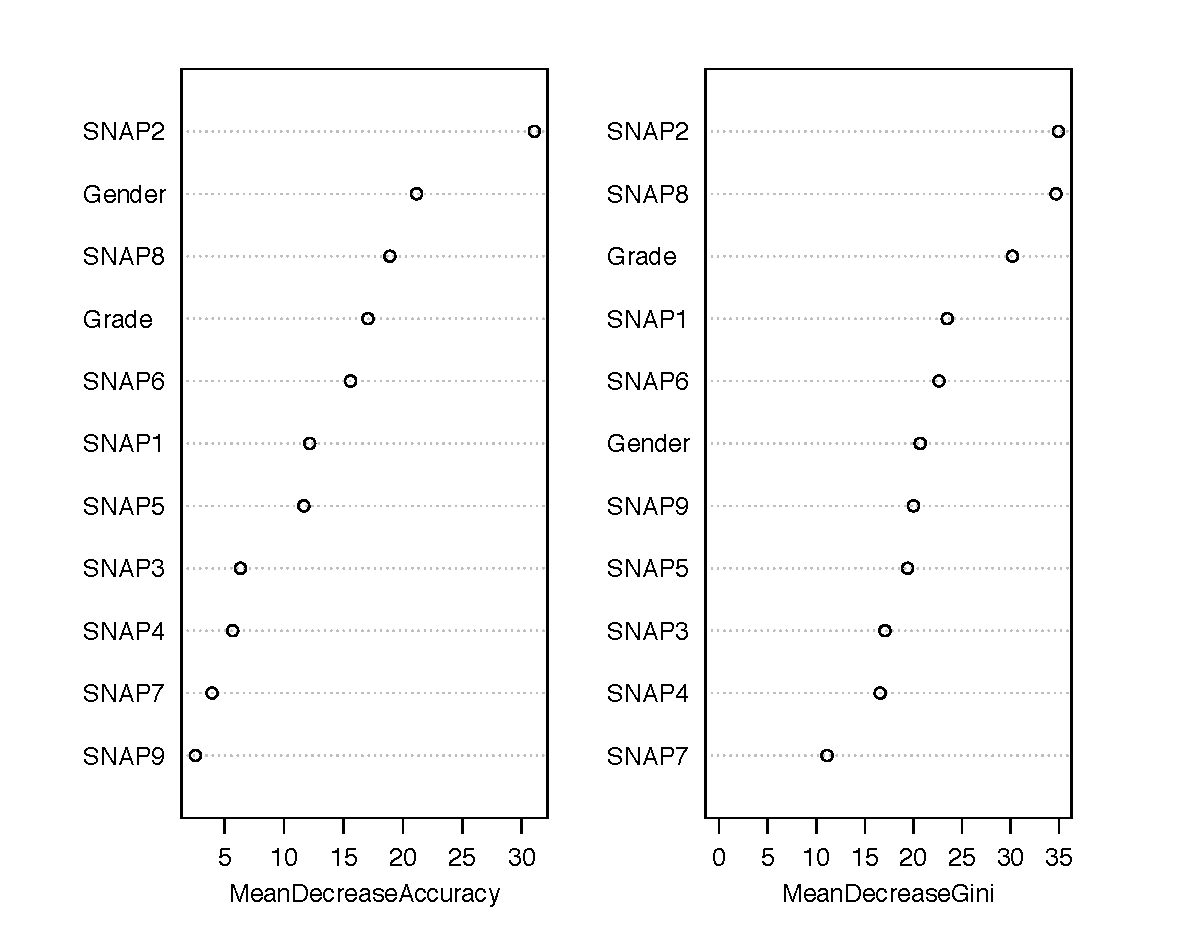
\includegraphics[width=0.85\textwidth]{./Figs/RF_variable_importance_pptx.pdf}
\caption{RF variable importance computed by  the {\tt importance()} function in the R package {\tt randomForest}}
\label{fig_rf_variable_importance}
\end{center}
\end{figure}


% The margin of a case is the proportion of votes for the true class minus the maximum proportion of votes for the other classes. 
% The size of the margin gives a measure of how confident the classification is.\\

Computing a measure of outlyingness for each case, based on a proximity matrix (explained in the Methods section), resulted in a numeric vector as
depicted in Figure~\ref{fig_rf_outlier_proximity}. These values are color-coded for academic achievement outcome in each case.
According to Breiman (2007), an outlyingness value above $10$ is reason to suspect the case of being outlying.

\begin{figure}[H]
\begin{center}
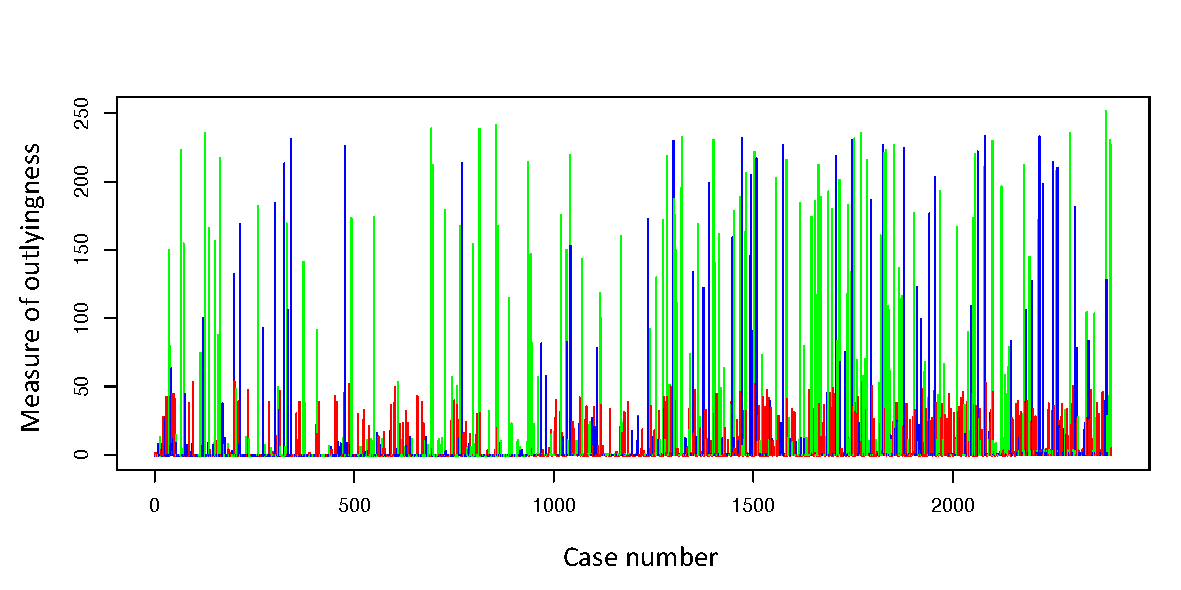
\includegraphics[width=0.95\textwidth]{./Figs/RF_outlier_proximity_pptx.pdf}
\caption{RF outlier measures computed by  the {\tt outlier()} function in the R package {\tt randomForest}. Colorcoding: red = {\it low}, 
green = {\it medium}, blue = {\it high}  academic achievement.}
\label{fig_rf_outlier_proximity}
\end{center}
\end{figure}

  
 A random forest regression including the three categories of achievement scores generated 500 trees was computed. The mean squared residuals was .483, and the explained 9.3\% of the variance in the academic achievement score in high school. The analysis also indicates the "importance" of variables (higher value means higher "importance"). The results (Table 4) select the item where teachers reported that the child \emph{often has difficulty sustaining attention in tasks or play activities}  as the most important, followed by class grade in primary school and the item reflecting that the teachers find that the child \emph{Often is distracted by extraneous stimuli}. However, the confusion matrix showed that the classification errors were high both for the medium and low academic achievement scores, while it is fairly good for the highest level. This shows the importance of running analyses including a high number of repetitions. Doubling the number of repetitions (n = 1000) did not change the "importance" of the single variables, but reduced the classification errors \\
 
 

  
  





\subsubsection*{Support vector machine (SVM)}



\subsubsection*{Artificial neural networks  (ANN)}



% \subsection*{Regression analysis including inattention items, gender and class grade in primary school}
%\begin{verbatim}
%## Multiple linear regression (using complete set of predictor variables)
%## lm(formula = ave ~ ., data = D)
%## 
%## Residuals:
%##     Min      1Q  Median      3Q     Max 
%## -3.2305 -0.4527  0.0403  0.4848  2.2817 
%## 
%## Coefficients:
%##              Estimate Std. Error t value Pr(>|t|)    
%## (Intercept)  4.230480   0.026481 159.756  < 2e-16 ***
%## genderBoy   -0.110695   0.029366  -3.770 0.000168 ***
%## grade3      -0.048591   0.032600  -1.490 0.136227    
%## grade4      -0.075571   0.036637  -2.063 0.039253 *  
%## tqSNAP11    -0.119047   0.048366  -2.461 0.013911 *  
%## tqSNAP21    -0.299222   0.065278  -4.584 4.80e-06 ***
%## tqSNAP31     0.021808   0.061564   0.354 0.723195    
%## tqSNAP41     0.026657   0.075502   0.353 0.724068    
%## tqSNAP51     0.009179   0.069739   0.132 0.895294    
%## tqSNAP61    -0.167617   0.068614  -2.443 0.014642 *  
%## tqSNAP71    -0.008221   0.090983  -0.090 0.928010    
%## tqSNAP81    -0.221153   0.042546  -5.198 2.19e-07 ***
%## tqSNAP91    -0.033856   0.054313  -0.623 0.533110    
%## ---
%## Signif. codes:  0 '***' 0.001 '**' 0.01 '*' 0.05 '.' 0.1 ' ' 1
%## 
%## Residual standard error: 0.6915 on 2384 degrees of freedom
%## Multiple R-squared:  0.1068, Adjusted R-squared:  0.1023 
%## F-statistic: 23.75 on 12 and 2384 DF,  p-value: < 2.2e-16\end{verbatim}
% 

% \subsection*{Recursive partitioning methods adding items reflecting externalizing behaviour}
% The regression tree was somewhat different, but did not include any of the items reflecting externalizing behaviour (Figure 3). MORE!
 
 % \subsection*{Neural network methods including inattention items, gender and class grade in primary school}


\section{DISCUSSION}

\subsection*{Summary of results}
The present study showed that inattention symptoms in early school years were not only frequently reported by teachers, but they did also contribute substantially to predict achievement in high-school nine years later.Inclusion of nine items reflecting different aspects of inattention in a multinominal regression analysis showed about a doubling of odds ratio for a low compared to high academic score for each extra score on items reflecting  behaviour reflecting problems with sustained attention (items 1, 2, 6) and distractibility (item 8). Inclusion of the nine items, gender and sex in the CART analysis revealed some interesting behavioural patterns and weights of the single variables. The first strongly significant item was related to how the child avoids, dislikes or is reluctant to take part in tasks that require sustained mental effort. As it was reported by primary school teachers, this was probably first of all related to school- and homework. Reports of distractibility turned out to be as important, both alone, but also when appearing together with problems related to sustained attention. A random forest regression analysis generating 500 decision trees confirmed sustained attention and distractibility to be the most important items in the decision tree. Although the model only explained 10\% of the variance and turned out to be the best predictor of the highest academic achievement level, the results should be carefully considered by teachers when detecting inattention problems in primary school children. \\


%Inattention in early childhood has been linked to a wide range of behavioral and social problems \cite{Bellanti2000, Connors2012}, with a fairly good documentation of a specific link to low academic attainment  \cite{Polderman2010, Pingault2014, Garner2013, Holmberg2014, Gray2014}. The present study contributed by using a statistical procedure generating decision trees revealing different weights associated with specific items and behavioural patterns. 
Some of our results clearly confirmed  findings in a study by Holmberg et al. \cite{Holmberg2014}, showing that teacher reports of failure to finish a task was one of the main factors in explaining academic outcome. In the present study, a more school- and homework related item was selected to have the strongest importance, but both variables are clearly related to the ability to sustain attention.  Our study add to Holmberg and collegueas' findings by revealing the importance of a behaviour pattern of inattention including distractibility.  Its relation to sustained attention in childhood is obvious, as a child with poor vigilance is expected to be disturbed by habits and disturbing cues in the environment. Taken together, these symptoms seem to represent the working memory and response inhibition problems described as hallmarks in several neuropsychiatric disorders, including ADHD \cite{Sonugabarke2005b}, and which are known to lead to a casscade of other problems \cite{Gillberg2010, Sonuga-Barke2010b}. When assessing sustained attention, one should therefore consider its association with distraction, as recently done in a study by Cassuto and collaborators \cite{Cassuto2013} including external distractors as part of a standard continuous performance test (CPT). But even children handling distractions in a standardized test situation may have problems in the classroom. Here, a child is expected to stay focused in a more disorganized situations with several external and internal distractors. When having difficulties in maintaining attention on a task, these distractors may be especially tempting. From experients in cognitive psychology we know that this is a challenge that is strongest in situations with high cognitive load \cite{Lavie2010}. Problems related to inattention are thus expected to be more hard to handle when a higher load is put on the curriculum in higher grades. \\

%This load is expected to be heavier in higher education than in primary school, emphasizing the importance of studies of developmental trajectories with repeated measures of inattention \cite{Pingault2014}. 





%Although obvious interactions at a behavioral level, there may still be differences on a biological leve as documented by Berry et al. \cite{Berry2014}. Interestingly, they related vulnerability of distraction to a genetic variant associated with depression \cite{Hahn2008}. Future studies should thus include prediction both to ADHD related and depression related problems in adolescents, not at least because there is obviously a strong overlap between these two problem areas in adolescents ( ). This was recently confirmed in a study based on the data included in the present study \cite{Lundervold2015}. Taken together, these results do not only inspiring development of non-pharmacological and pharmacological treatment efforts in adolescents, but also in primary school children vulnerable to distractibility and problems to sustain their attention in their school-related work.  
%Self-efficacy is known to play a key role in such a work related to academic achievement. In a study by Zadhone et al., \cite{Zahodne2011}, the association between executive function and self-efficacy was stronger in adults with low than high educational attainment. This indicates that improvement of self-efficacy should be included in remediation procedures for children reported to have executive dysfunctions. This has been demonstrated by programs incorporating strategies for self-efficacy enhancement (Catalano, Berglund, Ryan,
%Lonczak, Hawkins, 2004; Alfassi, 2003). This should be investigated in longitudinal studies, including both psychometric tests, as in Zahodne et al's study\cite{Zahodne2011}, but also by including teacher reports in primary school children as in the present study: teachers are probably the first to detect problems related to inattention, at least problems related to school-related work. \\
 
Girls were reported by their primary school teachers to have less inattention symptoms than boys, and they obtained significantly higher academic achievement scores in high school.  The importance of gender was, however, not as clear as expected when  the relation was investigated by the selected statistical procedures. These results suggests that the relation between the two variables was more gender balanced than measures of each of the two separately. \\


%The present result gives rise to speculations about the importance of cognitive function in primary school children. Distractibility is clearly related to response inhibition, which is commonly described as a which is described as  part of the concept of executive function \cite{Berger2013, Berger2015}.  It is well known that problems related to response inhibition may lead to a , and described as an important early factor in a hierarchical model of executive dysfunction in  ADHD \cite{Barkley1997b}. In this model, maturation is essential. For children with ADHD this seem to be delayed in childhood, with a gradual improvement during during adolescence (e.g., \cite{Faraone2006, Shaw2007b}), but these problems are not restricted to children with an ADHD diagnosis (\cite{Biederman} ?), and teachers' awareness and help to focus attention to obtain goals in school-related work will therefore be essential and probably also have a wide-ranged effect on future academic as well as occupational success. For clinicians, this should also be taken into account when assessing children with teacher-related problems related to sustained attention and distractibility.  The importance of distractors in the environment has led to a suggestion of using such distractors as part of the assessment evaluating if a child should be diagnosed with ADHD \cite{Cassuto2013}. From the present study, we suggest that this should be included also in children with symptoms that are subthreashold of ADHD. Our results showed the importance of a more detailed look at the different weights of problems related to inattention rather than being restricted by a diagnostic category.  \\


%
%In the present study we focused on the nine inattention symptoms that are part of the ADHD diagnosis. We are thus not dealing with a diagnostic category, but a dimension of symptoms that was shown to be of importance to educational attainment in high-school. Interestingly, distraction and sustained attention turned out to be identified as the main problems predicting achievement. Interestingly, Continuous Performance test is one of the main psychometric instruments used to assess problems related to ADHD, although clearly not valid as a diagnostic instrument. But valid as a test of sustained attention. Interestingly, extending the test by external distractions are shown to increase the validity of CPT to identify children with ADHD \cite{Cassuto2013}.  
%Although interaction effects make sense on a behavioral level, there may still be differences on a more basic biologiical level. This was documented by Berry et al. \cite{Berry2014}, relating a vulnerability of distraction to the cholinergic system (Ile89Val variant (rs1013940) of the CHT gene SLC5A7), a variant associated with depression \cite{Hahn2008} and the combined type of ADHD \cite{English2009}. This is consistent with previous studies showing strong overlap between symptoms of these two disorders in adolescents \cite{Lundervold2015}, calling for further studies of the relative importance of inattention symptoms and their interactions in samples with more severe symptoms of depression and ADHD. Taken together, the present findings and findings of biological markers of inattention symptoms suggest development of non-pharmacological and pharmacological treatment efforts to children in primary school vulnerable to distractibility and problems to sustain their attention in their school-related work.  \\\\


%
%
In the present study we included a statistical method that handle situations where predictor variables with a few number of categories may hide complex interactions. We thus found this method appropriate with our aim to investigate if specific problem areas are of importance to predict future academic outcome. Inattention is a complex concept, where the weights of different problem areas and their interactions may give information of importance to understand how to identify essential problems in a child. 
%Although one could argue that all problem areas are of importance, we assume that that is dependent on the selected outcome variable. Here, we focused on academic achievement, and future studies should include a wider range of variables to improve the overall explained variables. Here, the best explanation was found for the highest level, probably because lower academic scores are explained by a wider range of variables.By this, we still believe that the random forest method is more appropriate than more traditional linear regression model in predicting future function from previous reports of behavior know to disturb the child in a school situation. 
An alternative approach to cope with large numbers of predictor variables would be to first apply dimension reduction techniques, such as principle components or factor analysis, and then use standard regression methods on the reduced data set. However, this approach has the disadvantage that the original input variables are projected into a reduced set of components, so that their individual effect is no longer identifiable. As opposed to that, random forests can process large numbers of predictor variables simultaneously and provide individual measures of variable importance.
proves to be more stable than stepwise variable selection approaches available for logistic regression, which are known to be affected by order effects (see, e.g., Austin, Tu, 2004; Derksen \& Keselman, 1992; Freedman, 1983). By this and results from the present study, we argue for the appropriateness of this cluster of statistical methods when dealing with a multidimensional dataset and a high number of participants. \\


dicotomi
when these children were 16 to 19 years old high-school students. The  were cademic achievement is here obtained from an official registry wheHere we investigate if academic achievement in a population-based sample of Norwegian 16 - 19 years old high-school students can be classified from reports of inattention reports given by their primary teachers about 10 years earlier. As both age \cite{West2014}  and gender \cite{Gershon2002, Soerensen2008, Biederman2005} should be controlled for in studies focusing on inattention, they will both be added as predictors in the statistical analysis. \\



 \subsection*{Strengths and Limitations}
The large population-based sample of high-school students followed from childhood and inclusion of a standardized questionnaire assessing inattention and hyperactivity are two main strengths of the present study. A third strength was the inclusion of recursive partitioning methods to analyse our data. By this we could handle predictor variables with few categories and possible hided multidimensional interactions, and still generate behavioural patterns that was easy to interpret. \\

In spite of the strengths and the importance of the findings generated, several limitations must be mentioned. Although the statistical analyses have several strengths, applications of recursive partitioning methods in psychology also reveal common misperceptions and pitfalls. For example, Luellen et al. (2005) suspected that ensemble methods could overfit (i.e., adapt too closely to random variations in the learning sample).  By adding recursive partitioning, a high number of threes were generated. This is important, in that the selection of a splitting variable will strongly depend on the distribution in the learning sample. By repeating the procedure as in the present study, the prediction is expected to be more correct than when based on a single tree. \\\

Inclusion of very few predictor variables when assessing predictions over a nine-years period as in the present study, is another obvious limitation of the present study. A stronger model could have been obtained by including results from psychometric test assessing vigilance and distractibility, similar to the one developed by Cassuto et al. \cite{Cassuto2013}, or more ecological valid virtual reality test as the described by Pelham et al. \cite{Pelham2011}. Inclusion of only teacher reports may also be considered as a limitation. Although parent reports obviously are of importance, teacher reports were selected due to the focus of the present study and studies showing that teacher reports are stronger predictors of academic success than parent resports (). An even more sophisticated analysis would be to include repeated inattention measures to understand the trajectory from early symptoms of inattention to function in adolescence and adulthood. Its importance was shown in a study by Pingault and collaborators \cite{Pingault2014}, showing that increase in symptoms of inattention during childhood really matters when it comes to school graduation failure. Such studies are important and should include analysis of behavioural patterns, because a specific pattern of vigilance and distraction was suggested by the present study. \\


%
%The selection of inattention measures did also influence the result. We selected the nine items associated with an ADHD diagnosis. In the present study we focused on the nine inattention symptoms that are part of the ADHD diagnosis. We are thus not dealing with a diagnostic category, but a dimension of symptoms that was shown to be of importance to educational attainment in high-school. Interestingly, distraction and sustained attention turned out to be identified as the main problems predicting achievement. Interestingly, Continuous Performance test is one of the main psychometric instruments used to assess problems related to ADHD, although clearly not valid as a diagnostic instrument. But valid as a test of sustained attention. Interestingly, extending the test by external distractions are shown to increase the validity of CPT to identify children with ADHD \cite{Cassuto2013}. \\

%
%\subsubsection*{Future work}
% 
%Only about 10\% of the variance was explained by the inattention measures, leaving several other factors still unknown as predictors of later academic achievements. Such factors should be included in future studies. The importance of cognitive factors has already been mentioned, but a model should clearly take into account the mulitcontextual importance of  family, school, emotional, social and behavioural characteristics of the participants, as well as individual domains for adolescents' school success. Furthermore, there is a call for studies comparing results in countries with different attitudes and pressure on academic success. Large-scaled studies including a large number of participants and a wide range of variables should consider using the statistical methods advocated for in the present study, Based on findings of weights and behavioural patterns of important to educational success, there is a call for studies of remediation procedures for  problems related to inattention. .



\subsection*{Clinical and methodological implications and future directions}
Knowledge about the future function of children identified as inattentive by their primary school teachers should lead to remediation procedures. Poor inattention is not only predictive of poor academic outcome, but also linked to a wide range of other  present and future problems.The present study made us aware of the importance of a behavioural pattern including both the ability to sustain attention and to handle distractibility.  However, only about 10\% of the variance was explained by the inattention measures, leaving several other factors still unknown as predictors of later academic achievements that should be explored in future studies. The importance of cognitive factors has already been mentioned, but a model should clearly take into account the mulitcontextual importance of  family, school, emotional, social and behavioural characteristics of the participants, as well as individual domains for adolescents' school success. Furthermore, there is a call for studies comparing results in countries with different attitudes and pressure on academic success. Large-scaled studies including a large number of participants and a wide range of variables should consider using the statistical methods advocated for in the present study, Based on findings of weights and behavioural patterns of important to educational success, there is a call for studies of remediation procedures for  problems related to inattention. 

%
%Based on the results, further studies should be launched including a higher number of predictors. Different weighting is expected for most of the psychological outcome variables, as recently shown by Rosales in a study of the different weighst of the 18 ADHD symptoms to predict a diagnosis \cite{Rosales2015}. \\
%However, several limitations need to be commented on. First of all, to simplify the statistical model, we restricted our analysis to include very few variables.A higher explained variance and more complex behavioural patterns are expected if more variables were included.  \\
% It covers a cluster of methods turned out to be of importance to identify behavioural patterns in multidimentional predictors of inattention. 
%The introduction of a statistical procedure based on recursive partitioning methods was another main contribution of the present study.



\section*{Acknowledgments}

The present study was supported by the Centre for Child and Adolescent Mental Health and Welfare, Uni health, Uni Research, Bergen, Norway, and was also funded by the University of Bergen, the Norwegian Directorate for Health and Social Affairs, and the Western Norway Regional Health Authority. We are grateful to the children, parents and teachers participating in the Bergen Child Study (BCS) and members of the BCS project group for making the study possible.


%\end{doublespace}

\newpage
\bibliographystyle{apalike}

%\bibliography{depression}
\bibliography{bmc_article2}


\newpage

\end{document}


\begin{table}[H] 
\caption{The SNAP-IV items}
\label{SNAP_IV_items} 
\begin{small}
\begin{center}
\begin{tabular}{ll}
 \hline
 \bf{Inattention}\\ 
 \vspace{-5mm} \\
\bf{SNAP 1} & Often fails to give close attention to details or makes careless\\
 & mistakes in schoolwork, work, or other activities \\ 
\vspace{-5mm} \\
\bf{SNAP  2} & Often has difficulty sustaining attention in tasks or play activities \\ 
\vspace{-5mm} \\
\bf{SNAP  3} & Often does not seem to listen when spoken to directly \\ 
\vspace{-5mm} \\
\bf{SNAP  4} &  Often does not follow through on instructions and fails to finish \\
& schoolwork, chores, or duties  \\ 
\vspace{-5mm} \\
\bf{SNAP  5} & Often has difficulty organizing tasks and activities  \\ 
\vspace{-5mm} \\
\bf{SNAP  6} & Often avoids, dislikes, or is reluctant to engage in tasks that require\\
&  sustained mental effort  (e.g., schoolwork or homework) \\ 
\vspace{-5mm} \\
\bf{SNAP  7} & Often loses things necessary for tasks or activities (e.g., toys, school \\
& assignments, pencils, books, or tools) \\ 
\vspace{-5mm} \\
\bf{SNAP  8} & Often is distracted by extraneous stimuli \\ 
\vspace{-5mm} \\
\bf{SNAP  9} & Often is forgetful in daily activities \\ 
\vspace{-5mm} \\
\hline
 \bf{Hyperactivity}\\ 
 \vspace{-2mm} \\
 \bf{SNAP  10} & Often fidgets with hands or feet or squirms in seat\\
\vspace{-2mm} \\
\bf{SNAP  11} & Often leaves seat in classroom or in other situations in which remaining \\
& seated is expected\\ 
\vspace{-2mm} \\
\bf{SNAP  12} & Often runs about or climbs excessively in situations in which it is inappropriate \\ 
\vspace{-2mm} \\
\bf{SNAP  13} &  Often has difficulty playing or engaging in leisure activities quietly \\
\vspace{-2mm} \\
\bf{SNAP  14} & Often is "on the go" or often acts as if "driven by a motor"  \\ 
\vspace{-2mm} \\
\bf{SNAP  15} & Often talks exessively\\
\vspace{-2mm} \\
\bf{SNAP  16} & Often blurts out answers before questions have been completed\\ 
\vspace{-2mm} \\
\bf{SNAP  17} & Often has difficulty awaiting turn \\ 
\vspace{-2mm} \\
\bf{SNAP  18} & Often interrupts or intrudes on others (e.g., butts into conversations/games) \\ 
\vspace{-2mm} \\
\hline
\end{tabular}
\end{center}
\end{small}
\end{table}

%\subsection*{Table 1 - Results on the main measures in participants and non-participants}
% 
%\begin{table}[ht]
%\begin{center}
%\begin{tabular}{lrrrrrrrr}
%
%  \hline
%                & \multicolumn{2}{c}{\emph{Excluded}}  &  \multicolumn{2}{c}{\emph{Participants}}\\
%                    & Girls & Boys & Girls & Boys\\ 
% \hline                   
%      
%    Sex  & 64 & 116 & 43 & 84 \\ 
%    ASRS & 29.8 (8.4) & 23.8 (8.4) & 30.4 (10.8) &  27.3 (10.2)\\ 
%    ASRS Inattention  & 15.8 (5.5) & 12.7 (5.4) & 17.3 (5.8) & 15.6 (5.6) \\ 
%    sMFQ  &  8.5 (6.0)   & 4.8 (3.1)&*6.7 (5.5) & 4.4 (4.5) \\ 
%    Verbal Comprehension   & 89.2 (15.2)  & 86.5 (17.1) & 91.9 (12.8) & 92.1 (14.9)\\ 
%    Perceptual Organization & @92.7 (20.6)  & 90.0 (19.0) & *101.3 (14.0) & 93.9 (14.9) \\ 
%    Freedom from Distractability  & @92.2 (17.1) & 88.9 (19.7) & *99.2 (13.5) & 92.9 (17.5)   \\ 
%    Processing Speed  & 96.4 (17.7)  & 84.7 (19.2)  & **101.4 (19.2) & 86.4 (15.7) \\ 
%    FSIQ  & @88.9 (19.8) & 86.5 (17.1) & 96.2 (13.0) & 90.8 (15.5) \\ 
%
%    
%   \hline
%\end{tabular}
%\end{center}
%** p $<$ 0.001, * p $<$ 0.05 : Between the groups of girls and boys who participated; @p $<$ 0.05: Between the groups of excluded and participants. 
%\end{table}
%
%
%\newpage
%%
% \subsection*{Table 2 - Percentage of girls (N = 4466) and boys (N = 5148) with a given response on the items of ASRS}
% 
%\begin{table}[ht]
%\begin{center}
%\begin{tabular}{lrrrrrrrrrrr}
%
%  \hline
%                & \multicolumn{2}{c}{\emph{Never}}  &  \multicolumn{2}{c}{\emph{Rarely}}  & \multicolumn{2}{c}{\emph{Sometimes}} &\multicolumn{2}{c}{\emph{Often}} & \multicolumn{2}{c}{\emph{Very often}} &\\
%                    & Girls & Boys & Girls & Boys & Girls & Boys & Girls & Boys & Girls &Boys & OR***\\ 
% \hline                   
%      
%    Item 1*  & 7.2 & 13.5 & 28.2& 33.0 & 42.1 & 37.8 & 17.0 & 11.5 & 5.5 & 4.2  & 1.4\\ 15.7   6.9
%    Item 2*  & 14.9& 19.6 & 42.2 & 42.4 & 30.0 & 28.2 &9.8 & 7.0 & 3.1 & 2.7 & 1.33\\ 
%    Item 3*  & 19.1 & 20.4& 49.0 & 45.3 & 22,0 & 24.8 &7.4 & 7.3 & 2.5 & 2.2 & 1.03  \\ 
%    Item 4*  & 5.6  & 12.5 & 22.9 & 29.0 & 37.0 & 34.5 &24.8 & 17.2 & 9.7 & 6.7 & 1.44\\ 
%    Item 5**  & 5.2 & 9.6 & 15.0 & 17.6 & 28.5& 29.7 &31.3 & 25.7 & 20.0 & 17.5 & 1.19 \\ 
%     Item 6**  & 23.7 & 26.6 & 36.5 & 32.8 & 27.2 & 27.9 &9.0 &8.1 & 3.6 & 4.5 & 1.00\\ 
%     \hline
%     Item 7*  & 4.2 & 8.4 & 24.8 & 26.1 & 44.4 & 39.5 &20.0 & 18.4 & 6.5 & 6.5  & 1.06\\
%     Item 8*  & 2.8 & 8.2 & 14.2 & 20.6 & 39.5 & 37.3 & 30.4 & 23.1 & 13.1 & 10.9 & 1.28\\ 
%     Item 9* & 19.0  & 28.6 & 41.0 & 40.9 & 27.4 & 22.3 & 9.1 &5.9 & 3.4 & 2.2 & 1.53\\ 
%    Item 10* & 10.3 & 16.3 & 37.6 & 40.8 & 33.4 & 31.4 & 13.9& 8.4 & 4.9 & 3.1 & 1.64 \\
%    Item 11*  & 7.0 & 13.6 & 29.3 & 35.8 & 37.8 & 34.6 & 18.5& 11.6 & 7.4 & 4.4 & 1.61\\
%    Item 12**  & 52.4 & 54.8 & 34.7 & 33.4 & 10.4 & 9.4 & 1.9& 1.5 & 0.7 & 0.9 & 1.04\\
%    Item 13**  & 6.0&  13.3 & 27.4 & 29.8 & 42.8 & 35.6 & 17.4 & 14.4 & 6.4 & 6.8 & 1.13\\
%    Item 14**  & 26.3 & 38.6 & 36.6 &  35.6 & 21.5 & 16.4 & 11.3 & 6.6 & 4.3 &  2.8 & 1.66\\
%    Item 15**  & 13.2 & 22.3 & 38.0 & 42.9 & 34.1 & 25.8  & 10.9 & 6.3 & 3.9 & 2.7 & 1.63\\
%     Item 16**  & 21.2 & 33.0 & 44.3 & 41.4 & 27.0 & 20.1 & 5.6 & 3.6 & 2.7 & 1.9 & 1.35\\
%     Item 17**  & 30.7 & 37.0 & 44.2 & 41.1 & 20.2 & 17.0 & 3.7 & 3.4 & 1.1 & 1.6 & 0.98 \\
%     Item 18**  & 16.4 & 22.1 & 55.8 & 54.9 & 23.2 & 19.4 & 3.5 & 2.4 & 0.9 & 1.2  & 1.23 \\
%     \hline
%%     Item +1  & 72.3 & 84.3 & 20.1 & 12.1 & 7.6 & 3.6** && 2.1  \\
%%    Item +2 & 72.3 & 84.3 & 20.1 & 12.1 & 7.6 & 3.6** && 2.1  \\  
%%    Item +3  & 72.3 & 84.3 & 20.1 & 12.1 & 7.6 & 3.6** && 2.1  \\
%%    Item +4  & 72.3 & 84.3 & 20.1 & 12.1 & 7.6 & 3.6** && 2.1  \\
%%     Item +5  & 72.3 & 84.3 & 20.1 & 12.1 & 7.6 & 3.6** && 2.1  \\
%%     Item +6  & 72.3 & 84.3 & 20.1 & 12.1 & 7.6 & 3.6** && 2.1  \\
%%    
%\end{tabular}
%\end{center}
%* Inattention items
%** Hyperactivity-impulsivity items; ***OR = The girl:ratio of using the Often or Very often compared to the three other response categories. 
%\end{table}


%
%\subsection*{Table 1 - SMFQ and ASRS sum-scores in girls and boys}
%\begin{table}[H] 
%\begin{center}
%\begin{tabular}{lrrr}
%\hline
% & Girls & Boys & $d$ \\ 
%\hline
%Inattention scale teachers &\\
%Inattention scale parents & \\
%SMFQ sum & 7.4 (6.1) & 4.2 (4.9)** & .58 \\
%%ASRS sum  & 28.5 (10.1) & 25.1 (10.9)** & .32\\  
%ASRS Inattention & 15.9 (6.0) & 14.0 (6.4)** & .31\\
%%ASRS HypImp & 12.6 (5.3) & 11.1 (5.7)**  & .28\\
%Academic achievement &\\
%%ASRS Screener & 10.4 (4.1) & 9.5 (4.4)** & .21\\
%\hline
%%SMFQ category@ & 1.7 (2.8) & 0.8 (1.9)** & .38\\
%%%%SMFQ sometimes+always & 5.7 (3.8) & 3.4 (3.5)** &  \\
%%ASRS sum category  & 4.4 (3.2) & 3.6 (2.9)** & .26\\  
%%ASRS Inattention category & 2.1 (2.2) & 1.5 (2.0)** & 29\\
%%ASRS HypImp category & 2.3 (1.4) & 2.1 (1.4)**  & .14\\
%%ASRS Screener category & 1.4 (1.4) & 1.1 (1.3)** & .22 \\
%%\hline
%\end{tabular}
%\end{center}
% *HypImp = Hyperativity-impulsivity subscale; ** $p$$<$.001.
%\end{table}   
%
%%
%\newpage
%
%\subsection*{Table 2 - Means and standard deviations on the Inattention scales}
% 
%\begin{table}[ht]
%\begin{center}
%\begin{tabular}{lrrrrrr}
%
%  \hline
%                & \multicolumn{2}{c}{\emph{Teachers}}  &  \multicolumn{2}{c}{\emph{Parents}} &  \multicolumn{2}{c}{\emph{Self reports}}\\
%                    & Girls & Boys & Girls & Boys & Boys & Girls\\ 
% \hline                   
%      
%    Item 1  & 20.5 & 12.1 & 22.6 & 15.7\\ 
%    Item 2  &12.1 & 6.2 & 13.0 & 9.7\\ 
%    Item 3  & 26.0 & 12.2 & 9.8 & 9.5\\ 
%    Item 4  & 14.2 & 10.2 &  34.5 & 23.9\\ 
%    Item 5  & 14.0 & 5.8 & 51.3 & 43.1 \\ 
%     Item 6  & 11.0 & 2.0 & 12.6 & 12.6\\ 
%     Item 7  & 19.9 & 9.3  & 26.5 & 24.9\\ 
%     Item 8  & 8.3 & 3.2  & 43.5 & 33.9\\ 
%     Item 9  & 8.4 & 3.6 & 12.5 & 8.2\\ 
%%    Item 10 & 15.1 & 7.1 & 18.7 & 11.5 \\
%%    Item 11  & 7.3 & 3.7 & 25.8 & 16.0\\
%%    Item 12  & 10.5 & 4.7 & 2.5 & 2.4\\
%%    Item 13  & 7.6 & 3.6 & 23.9 & 21.2 \\
%%    Item 14 &&& 15.6 & 9.4\\
%%    Item 15 &&& 14.7 & 9.0\\
%%    Item 16 &&& 7.5 & 5.6 \\
%%    Item 17 &&& 4.8 & 4.9\\
%%    Item 18 &&& 4.4 & 3.6\\
%    
%    
%   \hline
%\end{tabular}
%\end{center}
%%** p $<$ 0.001: Report of \emph{True} from girls on an item compared to this report from boys\\
%%OR = Odds-ratios for girls to report \emph{True} compared to boys
%\end{table}
%
%\newpage
%%
%\subsection*{Table 3 - Number of severe ASRS items in the adolescents with an sMFQ score equal to or above 90th percentile}
%\begin{table}[H] 
%\begin{center}
%\begin{tabular}{lrrrrrrrrr}
%\hline
%& &  sMFQ high  & &  & sMFQ low  & &  \\
%&&(n=1098)&&&(n=8516)&&\\
% & All & Girls & Boys & All & Girls & Boys \\ 
%\hline
%ASRS sum  & 6.95 (3.73)* & 6.97 (3.59)* & 6.90 (4.17)* & 3.66 (2.77) & 3.89 (2.80) & 3.43 (2.73)\\  
%ASRS Inattention & 3.66 (2.61)* & 3.72 (2.57)* & 3.48 (2.74)* & 1.58 (1.91)  & 1.74 (1.97) & 1.42 (1.83)\\
%ASRS HypImp & 3.29 (1.71)* & 3.25 (1.65)* & 3.42 (1.92)* & 2.08 (1.30) & 2.15 (1.29) & 2.01 (1.31) \\
%%ASRS Screener & .45** & .35**\\
%%\hline
%%ASRS sum category  & .50** & .41**\\  
%%ASRS Inattention category & .46** & .39**\\
%%ASRS HypImp category & .38** & .36** \\
%%ASRS Screener category & .44** & .36**\\
%\hline
%\end{tabular}
%\end{center}
%SMFQcat1 = Always true response; SMFQcat2 = Sometimes true or Always true response;  HypImp = Hyperativity-impulsivity subscale; * $p$$<$.001,
%\end{table}   
%%

\newpage
\subsection*{Table 1 - Academic achievement scores according to the primary school and high school}
\begin{table}[H] 
\begin{center}
\begin{tabular}{lrrrrrr}
\hline

\hline
 & \multicolumn{3}{c}{\emph{Primary school class}}  &  \multicolumn{3}{c}{\emph{High school class}}\\
  & 2 & 3 & 4 & 1 & 2 & 3 \\ 
All  & 4.06 (.72) & 4.00 (.72) & 4.00 (.78) & 4.06 (.72) & 4.00 (.71) & 4.00 (.78) \\  
Girls & 4.18 (.74) & 4.11 (.70)  & 4.06 (.72) & 4.19 (.73) & 4.11 (.70) & 4.05 (.72)\\
Boys & 3.93 (.69) & 3.90 (.70) & 3.90  (.84) & 3.92 (.74) & 3.89 (.72) & 4.02 (.78)\\
\hline
\end{tabular}
\end{center}
%  ** $p$$<$.021 between the second and fourth primary school class,
\end{table}   


\newpage

%\subsection*{Table 2 - Percentage of children obtaining a given response from their teachers on each inattention item (SNAP-IV)}
% 
%\begin{table}[ht]
%\begin{center}
%\begin{tabular}{lrrlrrrrrr}
%
%  \hline
%                & \multicolumn{3}{c}{\emph{Not true}}  &  \multicolumn{3}{c}{\emph{Somewhat true}}\ &  \multicolumn{3}{c}{\emph{Certainly true}}\\
%                    & All & Girls & Boys  & All & Girls & Boys & All & Girls & Boys\\ 
% \hline                   
%      
%    SNAP 1  & 86.7 & 91.0 & 81.9**  & 11.3 & 7.6   & 15.4  & 2.0 & 1.3 & 2.7\\ 
%    SNAP 2  &88.3 & 93.9   & 82.1** & 9.6 & 5.6 & 14.0 & 2.1 & .5 & 3.9\\ 
%    SNAP 3  & 91.8  &  96.6 &  86.6** & 7.6 & 3.2 & 12.4 & .6 & .2 & 1.0 \\ 
%    SNAP 4  & 92.5  & 84.4   & 87.4**  & 6.8 & 3.6 & 10.4 & .7& .2 & 1.2 \\ 
%    SNAP 5  &  91.4 & 95.9 & 86.3**  & 7.3 & 3.6  & 11.5  &1.3 & .5 & 2.2  \\ 
%    SNAP 6  & 91.6 & 96.2 & 86.5**  & 7.1 & 3.4 & 11.5 & 1.3 & .4 & 2.4 \\ 
%    SNAP 7  & 96.5 & 98.5   & 94.2**   & 3.0  & 1.2 & 5.1& .5 & .3 & .7 \\ 
%    SNAP 8  & 74.8 & 84.3   & 64.4**  & 21.3  & 14.3  & 29.0 &  3.9 & 1.4 & 6.6\\ 
%    SNAP 9  & 89.4 & 93.3 & 85.0** & 9.5 & 6.3 & 13.1 & 1.1 & .4  & 1.9 \\ 
%        
%   \hline
%\end{tabular}
%\end{center}
%Total number of children = 2397, girls = 1256, boys = 1141. \\
%**: $p$ value $<$.001 according to ac chi-square test comparing a "not true" report in boys and girs
%\end{table}
%
%\newpage
%
%



%\newpage
%MAA LAGE NY TABELL MED NYE TALL
%\subsection*{Table 4 - Correlations between SMFQ scores and the ASRS scores in girls and boys}
%\begin{table}[H] 
%\begin{center}
%\begin{tabular}{lrr}
%\hline
%SMFQsum & Girls & Boys \\ 
%\hline
%ASRS sum  & .48** & .41**\\  
%ASRS Inattention & .47** & .38**\\
%ASRS HypImp & .39** & .36** \\
%%ASRS Screener & .45** & .35**\\
%\hline
%SMFQcat & Girls & Boys \\ 
%\hline
%ASRS sum category  & .45** & .36**\\  
%ASRS Inattention category & .42** & .33**\\
%ASRS HypImp category & .35** & .31** \\
%ASRS Screener category & .44** & .36**\\
%\hline
%\end{tabular}
%\end{center}
%SMFQcat = Always true response; HypImp = Hyperativity-impulsivity subscale; ** $p$$<$.001,
%\end{table}   



%\newpage
%
%%
%\subsection*{Table 3- Percentages with severe pain}
% \begin{table}[H]   
%%\begin{center}
%\begin{tabular}{lrrrr}
%\hline
%%%Independent variables\\
%Pain domain & All  & N & Girls & Boys\\
%\hline
%Headache  & 5.9 & 567 &  8.9 & 2.4\\
%Stomack ache & 4.4 & 421 & 6.1 & 2.4\\
%Back pain &  8.2 & 392  & 10.9 & 5.2\\
%Neck and Shoulder pain & 10.2& 977 &  15.1& 4.5\\
%\hline
%Number of pain domains\\
%\hline
%1  & 9.7 & 935 &  12.8 & 6.2 \\
%2 & 5.3 & 510 & 7.8 & 2.4 \\
%3 &  1.5 & 148  & 2.6 &0.3 \\
%4 & .9  & 86 & 1.2 & 0.6 \\
%\hline
%\end{tabular}
%%\end{center}
%%*Estimated regression coefficients: 
%%IB=intercept difference between boys and girls; ASRS=change in ASRS score with girls as a reference; ASRS:B= the ASRS-related effect for boys added to the ASRS change with girls as a reference. 
%\end{table}
%%
%\newpage
%
\
%
%\newpage
%\subsection*{Table 4- Prediction of academic achievement from gender and teacher and parent reported inattention symptom}
% \begin{table}[H]   
%\begin{center}
%\begin{tabular}{lrlrrlll}
%\hline
%%Independent variables\\
% \emph{sMFQ sum }\\
% & F-test & $df$ &  $p$-value & $R$$^2$ & I:B*&  Change:F* & Change:B*\\
%\hline
%Teachers\\
%Item 1  & 1220.0 & 3/9610 &  $<$.001 & .28 &  -1.66 &  .94*** &  .73***\\
%Item 2 & 1067.0 & 3/9610 & $<$.001 & .25 & -2.13*** &  1.26 ***  & .98*** \\
%Item 3 &   800.1 & 3/9610  & $<$.001 & .20 &  -2.00** &  1.62*** & 1.22***  \\
%Item 4  & 1167.0 & 3/9610 &  $<$0.001 & 0.27 &  0.35 & 0.29 &  -0.10\\
%Item 5 & 1081.0 & 3/9610 & $<$0.001 & 0.25 &    0.21  & 0.47 &  - 0.18\\
%Item 6 &   838.2 & 3/9610  & $<$0.001 &0.21 &  -1.09 &  0.45 & -0.13  \\
%Item 7  & 995.3 & 3/9610 &  $<$0.001 & 0.24 & -0.05 & 0.67 & -0.27\\
%Item 8   & 854.2 & 3/9610 &  $<$.001 & 0.21 &  -0.11 & 0.39*** &  0.24***\\
%Item 9 & 727.4 & 3/9610 & $<$.001 & 0.19 & -0.38*** &    0.52***  & 0.32** \\
%\hline
%Parents\\
%Item 1  & 1220.0 & 3/9610 &  $<$.001 & .28 &  -1.66 &  .94*** &  .73***\\
%Item 2 & 1067.0 & 3/9610 & $<$.001 & .25 & -2.13*** &  1.26 ***  & .98*** \\
%Item 3 &   800.1 & 3/9610  & $<$.001 & .20 &  -2.00** &  1.62*** & 1.22***  \\
%Item 4  & 1167.0 & 3/9610 &  $<$0.001 & 0.27 &  0.35 & 0.29 &  -0.10\\
%Item 5 & 1081.0 & 3/9610 & $<$0.001 & 0.25 &    0.21  & 0.47 &  - 0.18\\
%Item 6 &   838.2 & 3/9610  & $<$0.001 &0.21 &  -1.09 &  0.45 & -0.13  \\
%Item 7  & 995.3 & 3/9610 &  $<$0.001 & 0.24 & -0.05 & 0.67 & -0.27\\
%Item 8   & 854.2 & 3/9610 &  $<$.001 & 0.21 &  -0.11 & 0.39*** &  0.24***\\
%Item 9 & 727.4 & 3/9610 & $<$.001 & 0.19 & -0.38*** &    0.52***  & 0.32** \\
%\hline
%\end{tabular}
%\end{center}
%*Estimated regression coefficients: 
%IB=intercept difference between boys and girls; Change:F=change in score on the dependent variable with girls as a reference; Change:B= change in score for boys \\
%**: $p$ value $<$.05; ***: $p$ value $<$.001
%\end{table}
%
%\newpage

%
%\newpage
%\subsection*{Table 4 - Distribution of problem scores on the sMFQ and ASRS among adolescents visiting their GPs}
% 
%\begin{table}[ht]
%\begin{center}
%\begin{tabular}{lrrrrrrrrrr}
%
%  \hline
%                & \multicolumn{2}{c}{\emph{Mean (SD)}}  &  \multicolumn{2}{c}{\emph{75\%}} &  \multicolumn{2}{c}{\emph{85\%}}&  \multicolumn{2}{c}{\emph{90\%}} & \multicolumn{2}{c}{\emph{95\%}}\\
%                    & Girls & Boys & Girls & Boys & Girls & Boys & Girls & Boys & Girls & Boys\\ 
% \hline                   
%      
%    sMFQ  & 1.9 (2.9) & .9 (2.0) & 3 & 1 &5 & 2& 6 & 3 & 8 &5 \\ 
%    ASRS Sum  & 4.7 (3.3) & 4.0 (2.9) & 7 & 6 & 8 & 7 & 9 & 8 & 11 & 10 \\ 
%    ASRS Inattention  & 2.3 (2.3) & 1.7 (2.1) & 4 & 3 & 5 & 4& 6 & 4 & 7 & 6 \\ \ 
%    ASRS Hyp-Imp  & 2.5 (1.5) & 2.3 (1.4) & 3 & 3 & 4 & 4 & 5 & 4 & 5 & 5 \\ 
%   \hline
%\end{tabular}
%\end{center}
%%** p $<$ 0.001: Report of \emph{True} from girls on an item compared to this report from boys\\
%%OR = Odds-ratios for girls to report \emph{True} compared to boys
%\end{table}
%
\subsection*{Table 2- Importance of inattention items and their  Node Impurity}
 \begin{table}[H]   
\begin{center}
\begin{tabular}{lrrrrrrr}
\hline
%Independent variables\\
         & low* & medium* & high* & Accuracy* & Gini *& MSE** &  NodePurity**\\
\hline
%\emph{Inattention items} \\
 Gender  & 4.29  & -10.13 &  30.14  &  23.11  & 20.25 &  119.32      &   19.01\\
 Grade & --6.07 & 14.35 &16.92   &             15.85  &          30.11 & 3.20   &      23.22\\
  SNAP 1 & -2.18  &-17.41 &28.23  &              12.39   &   23.60  &  9.42   &      22.16\\
  SNAP 2 &  -1.46  & -1.62 &31.22      &          28.51      &      34.68&  25.99   &      52.95\\
  SNAP 3 & -18.98 &  2.06 &21.41 &                6.51      &      17.37& 11.20        & 14.85\\
  SNAP 4 &  -8.39  &-9.55& 21.32       &          7.31   &         16.51& 12.49     &    16.49\\
  SNAP 5 &  -9.41  &-1.14 &19.96     &           11.85     &       19.43 & 19.39     &    20.68\\
  SNAP 6 &  -13.87 & -2.30 & 28.55        &        14.67        &    21.76 & 14.58       &  22.09\\
  SNAP 7 & -3.92 &  -3.87 &10.62    &             2.68        &    11.06 &  5.77     &     8.12\\
  SNAP 8 &  1.05 &-23.88&37.12           &     19.69      &      34.68& 25.76     &    50.38\\
  SNAP 9 &  -7.60  & -1.86& 11.17&                 2.05    &        19.74&5.80   &      14.14\\
\hline
\end{tabular}
\end{center}
*Higher value means more important for low, medium and high academic achievements ; **Gini  shows the mean improvement in the splitting criteria for each variable, where higher values means higher importance; *** Impurity measure shows how much, over all trees, each split reduces node impurity, where higher values indicateds higher purity of a given measure. 
\end{table}

\newpage





%\subsection*{Table S-1- The items of the sMFQ}
%
%\begin{table}[ht]
%\begin{center}
%\begin{tabular}{ll}
%  \hline
%  
%\bf{Item 1} & I felt miserable or unhappy \\ 
%\bf{Item 2} & I didn't enjoy anything \\ 
%\bf{Item 3} & I felt so tired I just sat around and did nothing \\ 
%\bf{Item 4} &  I was restless  \\ 
%\bf{Item 5} &  I felt I was no good any more  \\ 
%\bf{Item 6} & I cried a lot  \\ 
%\bf{Item 7} & I found it hard to think properly or concentrate \\ 
%\bf{Item 8} & I hated myself  \\ 
%\bf{Item 9} & I was a bad person \\ 
%\bf{Item 10} & I felt lonely \\ 
%\bf{Item 11} & I thought nobody really loved me  \\ 
%\bf{Item 12} & I though I could never be as good as other kids\\ 
%\bf{Item 13} & I did everything wrong\\ 
%
%  \hline
%\end{tabular}
%\end{center}
%\end{table}
%
%%
%%\newpage
%
%\newpage
%\section*{Tables}
%\subsection*{Table S-2- Items included in the ASRS}
%
%\begin{table}[ht]
%\begin{center}
%\begin{tabular}{llrrrrr}
%  \hline
%   
%\bf{Item 1} & Trouble wrapping up the final details of a project, once the challenging parts have been done?\\ 
%\bf{Item 2} & Difficulty getting things in order when you have to do a task that requires organization? \\ 
%\bf{Item 3} & Problems remembering appointments or obligations? \\ 
%\bf{Item 4} &  When you have a task that requires a lot of thought, how often do you avoid or delay getting started?\\ 
%\bf{Item 5} & Fidget or squirm with your hands or feet when you have to sit down for a long time?\\ 
%\bf{Item 6} & Feel overly active and compelled to do things, like you were driven by a motor?\\ 
%%\hline
%\bf{Item 7} & Make careless mistakes when you have to work on a boring or difficult project? \\ 
%\bf{Item 8} & Difficulty keeping your attention when you are doing boring or repetitive work? \\ 
%\bf{Item 9} & Difficulty concentrating on what people say to you, even when they are speaking to you directly? \\ 
%\bf{Item 10} & Misplace or have difficulty finding things at home or at work? \\ 
%\bf{Item 11} & Distracted by activity or noise around you? \\ 
%\bf{Item 12} & Leave your seat in meetings or other situations in which you are expected to remain seated? \\ 
%\bf{Item 13} &Feel restless or fidgety? \\ 
%\bf{Item 14} & Difficulty unwinding and relaxing when you have time to yourself?\\
%\bf{Item 15} & Find yourself talking too much when you are in social situations?\\
%\bf{Item 16} & When in a conversation, find yourself finishing the sentences before they can finish them themselves?\\
%\bf{Item 17} & Difficulty waiting your turn in situations when turn taking is required?\\
%\bf{Item 18} & Interrupt others when they are busy?\\
%\hline
%
%  \hline
%\end{tabular}
%\end{center}
%\end{table}
%\newpage
%\newpage

%
%\noindent FIGURE LEGENDS
%%
%\vspace{20mm}
%%
%\noindent




%
%
%
%
%\vspace{25mm}
%
%\begin{figure}[H]
%\centering
%\caption{}
%\vspace{50mm}
%\includegraphics[width=0.99\linewidth]{./Figs/Figure1.jpg}
%\label{faallmethodsallsubjects}
%\end{figure}
%


\newpage

\section*{Table S-1- The SNAP-IV items}
\begin{table}[h!] 
\begin{center}
\begin{tabular}{ll}
 \hline
 \bf{Inattention}\\ 
 \vspace{-2mm} \\
\bf{SNAP 1} & Often fails to give close attention to details or makes careless\\
 & mistakes in schoolwork, work, or other activities \\ 
\vspace{-2mm} \\
\bf{SNAP  2} & Often has difficulty sustaining attention in tasks or play activities \\ 
\vspace{-2mm} \\
\bf{SNAP  3} & Often does not seem to listen when spoken to directly \\ 
\vspace{-2mm} \\
\bf{SNAP  4} &  Often does not follow through on instructions and fails to finish \\
& schoolwork, chores, or duties  \\ 
\vspace{-2mm} \\
\bf{SNAP  5} & Often has difficulty organizing tasks and activities  \\ 
\vspace{-2mm} \\
\bf{SNAP  6} & Often avoids, dislikes, or is reluctant to engage in tasks that require\\
&  sustained mental effort  (e.g., schoolwork or homework) \\ 
\vspace{-2mm} \\
\bf{SNAP  7} & Often loses things necessary for tasks or activities (e.g., toys, school \\
& assignments, pencils, books, or tools) \\ 
\vspace{-2mm} \\
\bf{SNAP  8} & Often is distracted by extraneous stimuli \\ 
\vspace{-2mm} \\
\bf{SNAP  9} & Often is forgetful in daily activities \\ 
\vspace{-2mm} \\
%\hline
% \bf{Hyperactivity}\\ 
% \vspace{-2mm} \\
% \bf{SNAP  10} & Often fidgets with hands or feet or squirms in seat\\
%\vspace{-2mm} \\
%\bf{SNAP  11} & Often leaves seat in classroom or in other situations in which remaining \\
%& seated is expected\\ 
%\vspace{-2mm} \\
%\bf{SNAP  12} & Often runs about or climbs excessively in situations in which it is inappropriate \\ 
%\vspace{-2mm} \\
%\bf{SNAP  13} &  Often has difficulty playing or engaging in leisure activities quietly \\
%\vspace{-2mm} \\
%\bf{SNAP  14} & Often is "on the go" or often acts as if "driven by a motor"  \\ 
%\vspace{-2mm} \\
%\bf{SNAP  15} & Often talks exessively\\
%\vspace{-2mm} \\
%\bf{SNAP  16} & Often blurts out answers before questions have been completed\\ 
%\vspace{-2mm} \\
%\bf{SNAP  17} & Often has difficulty awaiting turn \\ 
%\vspace{-2mm} \\
%\bf{SNAP  18} & Often interrupts or intrudes on others (e.g., butts into conversations/games) \\ 
%\vspace{-2mm} \\
\hline
\end{tabular}
\end{center}
\end{table}


% \end{doublespace}
%\end{frontmatter}

\end{document}

\newpage

\begin{tiny}
\begin{shaded}
\noindent {\scriptsize \underline{\textbackslash\!verbatiminput\{{\tt /Users/arvid/Dropbox/Arvid\_Inattention/code/astri\_wave1\_inattention\_cond\_infer\_trees\_20150626.Rmd}\}:}}
\verbatiminput{/Users/arvid/Dropbox/Arvid_Inattention/code/astri_wave1_inattention_cond_infer_trees_20150626.Rmd}
\end{shaded}
\end{tiny}


\end{document}
